\documentclass[a4paper]{book}
\usepackage{makeidx}
\usepackage{natbib}
\usepackage{graphicx}
\usepackage{multicol}
\usepackage{float}
\usepackage{listings}
\usepackage{color}
\usepackage{ifthen}
\usepackage[table]{xcolor}
\usepackage{textcomp}
\usepackage{alltt}
\usepackage{ifpdf}
\ifpdf
\usepackage[pdftex,
            pagebackref=true,
            colorlinks=true,
            linkcolor=blue,
            unicode
           ]{hyperref}
\else
\usepackage[ps2pdf,
            pagebackref=true,
            colorlinks=true,
            linkcolor=blue,
            unicode
           ]{hyperref}
\usepackage{pspicture}
\fi
\usepackage[utf8]{inputenc}
\usepackage{mathptmx}
\usepackage[scaled=.90]{helvet}
\usepackage{courier}
\usepackage{sectsty}
\usepackage[titles]{tocloft}
\usepackage{doxygen}
\lstset{language=C++,inputencoding=utf8,basicstyle=\footnotesize,breaklines=true,breakatwhitespace=true,tabsize=8,numbers=left }
\makeindex
\setcounter{tocdepth}{3}
\renewcommand{\footrulewidth}{0.4pt}
\renewcommand{\familydefault}{\sfdefault}
\hfuzz=15pt
\setlength{\emergencystretch}{15pt}
\hbadness=750
\tolerance=750
\begin{document}
\hypersetup{pageanchor=false,citecolor=blue}
\begin{titlepage}
\vspace*{7cm}
\begin{center}
{\Large \-Reference \-Manual}\\
\vspace*{1cm}
{\large \-Generated by Doxygen 1.7.6.1}\\
\vspace*{0.5cm}
{\small Thu May 2 2013 19:28:03}\\
\end{center}
\end{titlepage}
\clearemptydoublepage
\pagenumbering{roman}
\tableofcontents
\clearemptydoublepage
\pagenumbering{arabic}
\hypersetup{pageanchor=true,citecolor=blue}
\chapter{\-Class \-Index}
\section{\-Class \-Hierarchy}
\-This inheritance list is sorted roughly, but not completely, alphabetically\-:\begin{DoxyCompactList}
\item \contentsline{section}{\-Clock}{\pageref{classClock}}{}
\item \contentsline{section}{\-Operation}{\pageref{classOperation}}{}
\item \contentsline{section}{\-Operation\-File\-Parser}{\pageref{classOperationFileParser}}{}
\item \contentsline{section}{\-Operation\-List}{\pageref{classOperationList}}{}
\item \contentsline{section}{\-Register\-Files}{\pageref{classRegisterFiles}}{}
\item \contentsline{section}{\-Reservation\-Station}{\pageref{classReservationStation}}{}
\begin{DoxyCompactList}
\item \contentsline{section}{\-A\-L\-U\-Station}{\pageref{classALUStation}}{}
\item \contentsline{section}{\-Mem\-Station}{\pageref{classMemStation}}{}
\end{DoxyCompactList}
\item \contentsline{section}{\-Simulation}{\pageref{classSimulation}}{}
\item \contentsline{section}{\-Test\-Modules}{\pageref{classTestModules}}{}
\item \contentsline{section}{\-Tomasulo\-G\-U\-I}{\pageref{classTomasuloGUI}}{}
\end{DoxyCompactList}

\chapter{\-Class \-Index}
\section{Class List}
Here are the classes, structs, unions and interfaces with brief descriptions:\begin{DoxyCompactList}
\item\contentsline{section}{\hyperlink{classOperation}{Operation} }{\pageref{classOperation}}{}
\item\contentsline{section}{\hyperlink{classOperationFileParser}{OperationFileParser} }{\pageref{classOperationFileParser}}{}
\item\contentsline{section}{\hyperlink{classOperationList}{OperationList} }{\pageref{classOperationList}}{}
\item\contentsline{section}{\hyperlink{classRegisterFiles}{RegisterFiles} }{\pageref{classRegisterFiles}}{}
\end{DoxyCompactList}

\chapter{\-File \-Index}
\section{\-File \-List}
\-Here is a list of all files with brief descriptions\-:\begin{DoxyCompactList}
\item\contentsline{section}{\hyperlink{ALUStation_8java}{\-A\-L\-U\-Station.\-java} }{\pageref{ALUStation_8java}}{}
\item\contentsline{section}{\hyperlink{Clock_8java}{\-Clock.\-java} }{\pageref{Clock_8java}}{}
\item\contentsline{section}{\hyperlink{MemStation_8java}{\-Mem\-Station.\-java} }{\pageref{MemStation_8java}}{}
\item\contentsline{section}{\hyperlink{Operation_8java}{\-Operation.\-java} }{\pageref{Operation_8java}}{}
\item\contentsline{section}{\hyperlink{OperationFileParser_8java}{\-Operation\-File\-Parser.\-java} }{\pageref{OperationFileParser_8java}}{}
\item\contentsline{section}{\hyperlink{OperationList_8java}{\-Operation\-List.\-java} }{\pageref{OperationList_8java}}{}
\item\contentsline{section}{\hyperlink{RegisterFiles_8java}{\-Register\-Files.\-java} }{\pageref{RegisterFiles_8java}}{}
\item\contentsline{section}{\hyperlink{ReservationStation_8java}{\-Reservation\-Station.\-java} }{\pageref{ReservationStation_8java}}{}
\item\contentsline{section}{\hyperlink{Simulation_8java}{\-Simulation.\-java} }{\pageref{Simulation_8java}}{}
\item\contentsline{section}{\hyperlink{TestModules_8java}{\-Test\-Modules.\-java} }{\pageref{TestModules_8java}}{}
\item\contentsline{section}{\hyperlink{TomasuloGUI_8java}{\-Tomasulo\-G\-U\-I.\-java} }{\pageref{TomasuloGUI_8java}}{}
\end{DoxyCompactList}

\chapter{\-Class \-Documentation}
\hypertarget{classALUStation}{\section{\-A\-L\-U\-Station \-Class \-Reference}
\label{classALUStation}\index{\-A\-L\-U\-Station@{\-A\-L\-U\-Station}}
}
\-Inheritance diagram for \-A\-L\-U\-Station\-:\begin{figure}[H]
\begin{center}
\leavevmode
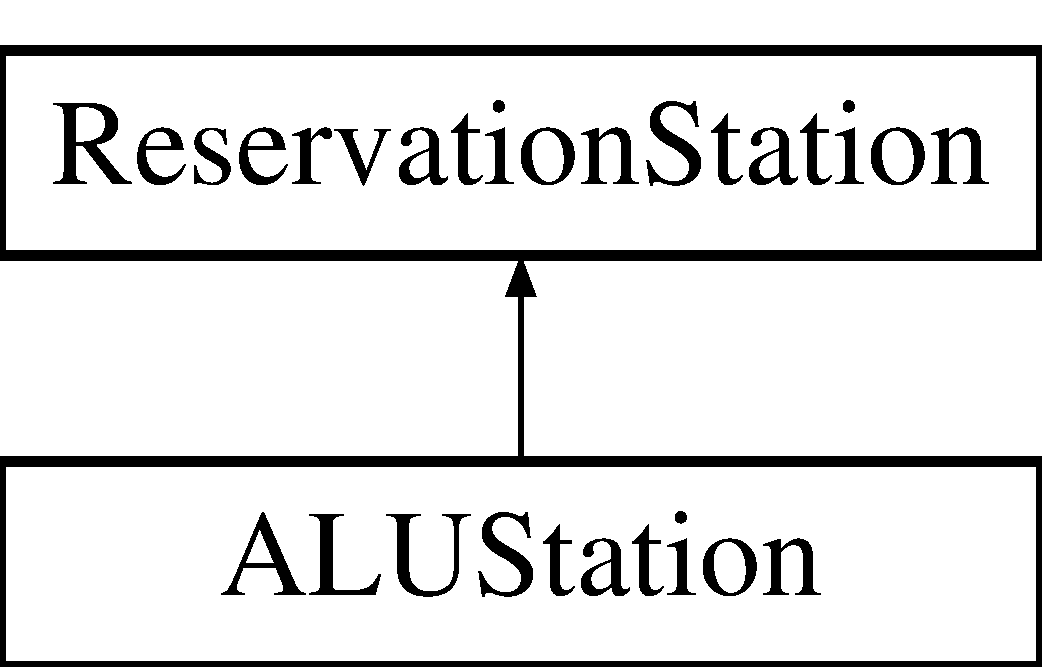
\includegraphics[height=2.000000cm]{classALUStation}
\end{center}
\end{figure}
\subsection*{\-Public \-Member \-Functions}
\begin{DoxyCompactItemize}
\item 
\hyperlink{classALUStation_ad072a1418f290945613c341e10e2790f}{\-A\-L\-U\-Station} (\-String \hyperlink{classReservationStation_a2c0bd5b95f126395b0ab081394f090f6}{sname})
\item 
void \hyperlink{classALUStation_a2fa486045af0a1ceea0cc089f1d7c285}{clear} ()
\item 
boolean \hyperlink{classALUStation_a5594f76ac16f7d0ee029759a8aa0e95b}{is\-Ready} ()
\item 
void \hyperlink{classALUStation_a7390a161d8b942caf223b17ea3c10eaf}{schedule\-Instruction} (\hyperlink{classOperation}{\-Operation} op, \hyperlink{classRegisterFiles}{\-Register\-Files} reg\-\_\-in, int cycles)
\item 
\-String \hyperlink{classALUStation_a3994abd08bd21c0909e618fccfa71232}{get\-Vj} ()
\item 
\-String \hyperlink{classALUStation_a9ccb24522168da4e49c73181713456c5}{get\-Vk} ()
\item 
\-String \hyperlink{classALUStation_ae0a7442f52e927afe64ea6d2c4c4ce35}{get\-Qj} ()
\item 
\-String \hyperlink{classALUStation_a37809dac94705eb79f8e86edd500df93}{get\-Qk} ()
\item 
\-String \hyperlink{classALUStation_a9fc599d8a1cc18e346f8906b89f99826}{get\-A} ()
\item 
void \hyperlink{classALUStation_a28b3efd541c418802585a67ff2c1ee4a}{set\-Qj} (\-String \hyperlink{classReservationStation_a2c0bd5b95f126395b0ab081394f090f6}{sname})
\item 
void \hyperlink{classALUStation_aa9c34c3462cf28b45ca0aee15720a6a7}{set\-Qk} (\-String \hyperlink{classReservationStation_a2c0bd5b95f126395b0ab081394f090f6}{sname})
\item 
void \hyperlink{classALUStation_af5cf876f7797834ded145c7d1399a9d6}{set\-Vj} (\-String i)
\item 
void \hyperlink{classALUStation_ab49be93fcb73de71abd3d26b8cad9d0d}{set\-Vk} (\-String i)
\item 
void \hyperlink{classALUStation_a3f3398c9971fcef712be2b1d30ef7fde}{set\-A} (\-String i)
\item 
\-String \hyperlink{classALUStation_a7e8a7ef42658641d2ec67f4c6284e4f7}{get\-Operation} ()
\end{DoxyCompactItemize}
\subsection*{\-Package \-Functions}
\begin{DoxyCompactItemize}
\item 
void \hyperlink{classALUStation_a07849653d1e2bc771def80de30ab24f2}{finalize\-Result} ()
\end{DoxyCompactItemize}
\subsection*{\-Private \-Attributes}
\begin{DoxyCompactItemize}
\item 
\-String \hyperlink{classALUStation_a1b7e9688731461f02ed6dba04f2c367b}{vj}
\begin{DoxyCompactList}\small\item\em value of operand \end{DoxyCompactList}\item 
\-String \hyperlink{classALUStation_aa9807e1058e78381d0682338bbf241fe}{vk}
\begin{DoxyCompactList}\small\item\em value of operand \end{DoxyCompactList}\item 
\-String \hyperlink{classALUStation_ad4f9bb91cc8aea34e2820692b053a6b9}{qj}
\begin{DoxyCompactList}\small\item\em name of reservation station producing \-Vj \end{DoxyCompactList}\item 
\-String \hyperlink{classALUStation_a4f5501e1bb07e37c0bfc884f6f19fdfa}{qk}
\begin{DoxyCompactList}\small\item\em name of reservation station producing \-Vk \end{DoxyCompactList}\item 
\-String \hyperlink{classALUStation_a8f2c76f7cdf676b26a20457f657d6083}{\-A}
\begin{DoxyCompactList}\small\item\em used to hold immediate field or off address \end{DoxyCompactList}\end{DoxyCompactItemize}


\subsection{\-Detailed \-Description}
\-This class provides all \hyperlink{classALUStation}{\-A\-L\-U\-Station} functionality. 

\subsection{\-Constructor \& \-Destructor \-Documentation}
\hypertarget{classALUStation_ad072a1418f290945613c341e10e2790f}{\index{\-A\-L\-U\-Station@{\-A\-L\-U\-Station}!\-A\-L\-U\-Station@{\-A\-L\-U\-Station}}
\index{\-A\-L\-U\-Station@{\-A\-L\-U\-Station}!ALUStation@{\-A\-L\-U\-Station}}
\subsubsection[{\-A\-L\-U\-Station}]{\setlength{\rightskip}{0pt plus 5cm}{\bf \-A\-L\-U\-Station.\-A\-L\-U\-Station} (
\begin{DoxyParamCaption}
\item[{\-String}]{sname}
\end{DoxyParamCaption}
)}}\label{classALUStation_ad072a1418f290945613c341e10e2790f}
\-Calls superclass constructor and initializes vj,vk,qj and qk 

\subsection{\-Member \-Function \-Documentation}
\hypertarget{classALUStation_a2fa486045af0a1ceea0cc089f1d7c285}{\index{\-A\-L\-U\-Station@{\-A\-L\-U\-Station}!clear@{clear}}
\index{clear@{clear}!ALUStation@{\-A\-L\-U\-Station}}
\subsubsection[{clear}]{\setlength{\rightskip}{0pt plus 5cm}void {\bf \-A\-L\-U\-Station.\-clear} (
\begin{DoxyParamCaption}
{}
\end{DoxyParamCaption}
)\hspace{0.3cm}{\ttfamily  \mbox{[}virtual\mbox{]}}}}\label{classALUStation_a2fa486045af0a1ceea0cc089f1d7c285}
\-Function to clear the \-Reservation \-Station 

\-Implements \hyperlink{classReservationStation_a5788893e16b640dc7edbab832b1cb80d}{\-Reservation\-Station}.

\hypertarget{classALUStation_a07849653d1e2bc771def80de30ab24f2}{\index{\-A\-L\-U\-Station@{\-A\-L\-U\-Station}!finalize\-Result@{finalize\-Result}}
\index{finalize\-Result@{finalize\-Result}!ALUStation@{\-A\-L\-U\-Station}}
\subsubsection[{finalize\-Result}]{\setlength{\rightskip}{0pt plus 5cm}void {\bf \-A\-L\-U\-Station.\-finalize\-Result} (
\begin{DoxyParamCaption}
{}
\end{DoxyParamCaption}
)\hspace{0.3cm}{\ttfamily  \mbox{[}package\mbox{]}}}}\label{classALUStation_a07849653d1e2bc771def80de30ab24f2}
\-Finalize the result -\/ perform integer parsing if necessary \hypertarget{classALUStation_a9fc599d8a1cc18e346f8906b89f99826}{\index{\-A\-L\-U\-Station@{\-A\-L\-U\-Station}!get\-A@{get\-A}}
\index{get\-A@{get\-A}!ALUStation@{\-A\-L\-U\-Station}}
\subsubsection[{get\-A}]{\setlength{\rightskip}{0pt plus 5cm}\-String {\bf \-A\-L\-U\-Station.\-get\-A} (
\begin{DoxyParamCaption}
{}
\end{DoxyParamCaption}
)}}\label{classALUStation_a9fc599d8a1cc18e346f8906b89f99826}
\-Function returns the value \-A \hypertarget{classALUStation_a7e8a7ef42658641d2ec67f4c6284e4f7}{\index{\-A\-L\-U\-Station@{\-A\-L\-U\-Station}!get\-Operation@{get\-Operation}}
\index{get\-Operation@{get\-Operation}!ALUStation@{\-A\-L\-U\-Station}}
\subsubsection[{get\-Operation}]{\setlength{\rightskip}{0pt plus 5cm}\-String {\bf \-A\-L\-U\-Station.\-get\-Operation} (
\begin{DoxyParamCaption}
{}
\end{DoxyParamCaption}
)}}\label{classALUStation_a7e8a7ef42658641d2ec67f4c6284e4f7}
\-Return an operation type descriptor \hypertarget{classALUStation_ae0a7442f52e927afe64ea6d2c4c4ce35}{\index{\-A\-L\-U\-Station@{\-A\-L\-U\-Station}!get\-Qj@{get\-Qj}}
\index{get\-Qj@{get\-Qj}!ALUStation@{\-A\-L\-U\-Station}}
\subsubsection[{get\-Qj}]{\setlength{\rightskip}{0pt plus 5cm}\-String {\bf \-A\-L\-U\-Station.\-get\-Qj} (
\begin{DoxyParamCaption}
{}
\end{DoxyParamCaption}
)}}\label{classALUStation_ae0a7442f52e927afe64ea6d2c4c4ce35}
\-Function returns the value qj \hypertarget{classALUStation_a37809dac94705eb79f8e86edd500df93}{\index{\-A\-L\-U\-Station@{\-A\-L\-U\-Station}!get\-Qk@{get\-Qk}}
\index{get\-Qk@{get\-Qk}!ALUStation@{\-A\-L\-U\-Station}}
\subsubsection[{get\-Qk}]{\setlength{\rightskip}{0pt plus 5cm}\-String {\bf \-A\-L\-U\-Station.\-get\-Qk} (
\begin{DoxyParamCaption}
{}
\end{DoxyParamCaption}
)}}\label{classALUStation_a37809dac94705eb79f8e86edd500df93}
\-Function returns the value qk \hypertarget{classALUStation_a3994abd08bd21c0909e618fccfa71232}{\index{\-A\-L\-U\-Station@{\-A\-L\-U\-Station}!get\-Vj@{get\-Vj}}
\index{get\-Vj@{get\-Vj}!ALUStation@{\-A\-L\-U\-Station}}
\subsubsection[{get\-Vj}]{\setlength{\rightskip}{0pt plus 5cm}\-String {\bf \-A\-L\-U\-Station.\-get\-Vj} (
\begin{DoxyParamCaption}
{}
\end{DoxyParamCaption}
)}}\label{classALUStation_a3994abd08bd21c0909e618fccfa71232}
\-Function returns the value vj \hypertarget{classALUStation_a9ccb24522168da4e49c73181713456c5}{\index{\-A\-L\-U\-Station@{\-A\-L\-U\-Station}!get\-Vk@{get\-Vk}}
\index{get\-Vk@{get\-Vk}!ALUStation@{\-A\-L\-U\-Station}}
\subsubsection[{get\-Vk}]{\setlength{\rightskip}{0pt plus 5cm}\-String {\bf \-A\-L\-U\-Station.\-get\-Vk} (
\begin{DoxyParamCaption}
{}
\end{DoxyParamCaption}
)}}\label{classALUStation_a9ccb24522168da4e49c73181713456c5}
\-Function returns the value vk \hypertarget{classALUStation_a5594f76ac16f7d0ee029759a8aa0e95b}{\index{\-A\-L\-U\-Station@{\-A\-L\-U\-Station}!is\-Ready@{is\-Ready}}
\index{is\-Ready@{is\-Ready}!ALUStation@{\-A\-L\-U\-Station}}
\subsubsection[{is\-Ready}]{\setlength{\rightskip}{0pt plus 5cm}boolean {\bf \-A\-L\-U\-Station.\-is\-Ready} (
\begin{DoxyParamCaption}
{}
\end{DoxyParamCaption}
)\hspace{0.3cm}{\ttfamily  \mbox{[}virtual\mbox{]}}}}\label{classALUStation_a5594f76ac16f7d0ee029759a8aa0e95b}
\-Function to determine whether operands are available and therefore ready for execution 

\-Implements \hyperlink{classReservationStation_a4fe26aca967123d4e9ec5aabf55d4d17}{\-Reservation\-Station}.

\hypertarget{classALUStation_a7390a161d8b942caf223b17ea3c10eaf}{\index{\-A\-L\-U\-Station@{\-A\-L\-U\-Station}!schedule\-Instruction@{schedule\-Instruction}}
\index{schedule\-Instruction@{schedule\-Instruction}!ALUStation@{\-A\-L\-U\-Station}}
\subsubsection[{schedule\-Instruction}]{\setlength{\rightskip}{0pt plus 5cm}void {\bf \-A\-L\-U\-Station.\-schedule\-Instruction} (
\begin{DoxyParamCaption}
\item[{{\bf \-Operation}}]{op, }
\item[{{\bf \-Register\-Files}}]{reg\-\_\-in, }
\item[{int}]{cycles}
\end{DoxyParamCaption}
)\hspace{0.3cm}{\ttfamily  \mbox{[}virtual\mbox{]}}}}\label{classALUStation_a7390a161d8b942caf223b17ea3c10eaf}
\-Function to schedule the instruction 

\-Implements \hyperlink{classReservationStation_a5108e433a0a7e7cdd072fa7bcecdd399}{\-Reservation\-Station}.

\hypertarget{classALUStation_a3f3398c9971fcef712be2b1d30ef7fde}{\index{\-A\-L\-U\-Station@{\-A\-L\-U\-Station}!set\-A@{set\-A}}
\index{set\-A@{set\-A}!ALUStation@{\-A\-L\-U\-Station}}
\subsubsection[{set\-A}]{\setlength{\rightskip}{0pt plus 5cm}void {\bf \-A\-L\-U\-Station.\-set\-A} (
\begin{DoxyParamCaption}
\item[{\-String}]{i}
\end{DoxyParamCaption}
)}}\label{classALUStation_a3f3398c9971fcef712be2b1d30ef7fde}
\-Function to set the value of \-A \hypertarget{classALUStation_a28b3efd541c418802585a67ff2c1ee4a}{\index{\-A\-L\-U\-Station@{\-A\-L\-U\-Station}!set\-Qj@{set\-Qj}}
\index{set\-Qj@{set\-Qj}!ALUStation@{\-A\-L\-U\-Station}}
\subsubsection[{set\-Qj}]{\setlength{\rightskip}{0pt plus 5cm}void {\bf \-A\-L\-U\-Station.\-set\-Qj} (
\begin{DoxyParamCaption}
\item[{\-String}]{sname}
\end{DoxyParamCaption}
)}}\label{classALUStation_a28b3efd541c418802585a67ff2c1ee4a}
\-Function to set the value of qj \hypertarget{classALUStation_aa9c34c3462cf28b45ca0aee15720a6a7}{\index{\-A\-L\-U\-Station@{\-A\-L\-U\-Station}!set\-Qk@{set\-Qk}}
\index{set\-Qk@{set\-Qk}!ALUStation@{\-A\-L\-U\-Station}}
\subsubsection[{set\-Qk}]{\setlength{\rightskip}{0pt plus 5cm}void {\bf \-A\-L\-U\-Station.\-set\-Qk} (
\begin{DoxyParamCaption}
\item[{\-String}]{sname}
\end{DoxyParamCaption}
)}}\label{classALUStation_aa9c34c3462cf28b45ca0aee15720a6a7}
\-Function to set the value of qk \hypertarget{classALUStation_af5cf876f7797834ded145c7d1399a9d6}{\index{\-A\-L\-U\-Station@{\-A\-L\-U\-Station}!set\-Vj@{set\-Vj}}
\index{set\-Vj@{set\-Vj}!ALUStation@{\-A\-L\-U\-Station}}
\subsubsection[{set\-Vj}]{\setlength{\rightskip}{0pt plus 5cm}void {\bf \-A\-L\-U\-Station.\-set\-Vj} (
\begin{DoxyParamCaption}
\item[{\-String}]{i}
\end{DoxyParamCaption}
)}}\label{classALUStation_af5cf876f7797834ded145c7d1399a9d6}
\-Function to set the value of vj \hypertarget{classALUStation_ab49be93fcb73de71abd3d26b8cad9d0d}{\index{\-A\-L\-U\-Station@{\-A\-L\-U\-Station}!set\-Vk@{set\-Vk}}
\index{set\-Vk@{set\-Vk}!ALUStation@{\-A\-L\-U\-Station}}
\subsubsection[{set\-Vk}]{\setlength{\rightskip}{0pt plus 5cm}void {\bf \-A\-L\-U\-Station.\-set\-Vk} (
\begin{DoxyParamCaption}
\item[{\-String}]{i}
\end{DoxyParamCaption}
)}}\label{classALUStation_ab49be93fcb73de71abd3d26b8cad9d0d}
\-Function to set the value of vk 

\subsection{\-Member \-Data \-Documentation}
\hypertarget{classALUStation_a8f2c76f7cdf676b26a20457f657d6083}{\index{\-A\-L\-U\-Station@{\-A\-L\-U\-Station}!\-A@{\-A}}
\index{\-A@{\-A}!ALUStation@{\-A\-L\-U\-Station}}
\subsubsection[{\-A}]{\setlength{\rightskip}{0pt plus 5cm}\-String {\bf \-A\-L\-U\-Station.\-A}\hspace{0.3cm}{\ttfamily  \mbox{[}private\mbox{]}}}}\label{classALUStation_a8f2c76f7cdf676b26a20457f657d6083}


used to hold immediate field or off address 

\hypertarget{classALUStation_ad4f9bb91cc8aea34e2820692b053a6b9}{\index{\-A\-L\-U\-Station@{\-A\-L\-U\-Station}!qj@{qj}}
\index{qj@{qj}!ALUStation@{\-A\-L\-U\-Station}}
\subsubsection[{qj}]{\setlength{\rightskip}{0pt plus 5cm}\-String {\bf \-A\-L\-U\-Station.\-qj}\hspace{0.3cm}{\ttfamily  \mbox{[}private\mbox{]}}}}\label{classALUStation_ad4f9bb91cc8aea34e2820692b053a6b9}


name of reservation station producing \-Vj 

\hypertarget{classALUStation_a4f5501e1bb07e37c0bfc884f6f19fdfa}{\index{\-A\-L\-U\-Station@{\-A\-L\-U\-Station}!qk@{qk}}
\index{qk@{qk}!ALUStation@{\-A\-L\-U\-Station}}
\subsubsection[{qk}]{\setlength{\rightskip}{0pt plus 5cm}\-String {\bf \-A\-L\-U\-Station.\-qk}\hspace{0.3cm}{\ttfamily  \mbox{[}private\mbox{]}}}}\label{classALUStation_a4f5501e1bb07e37c0bfc884f6f19fdfa}


name of reservation station producing \-Vk 

\hypertarget{classALUStation_a1b7e9688731461f02ed6dba04f2c367b}{\index{\-A\-L\-U\-Station@{\-A\-L\-U\-Station}!vj@{vj}}
\index{vj@{vj}!ALUStation@{\-A\-L\-U\-Station}}
\subsubsection[{vj}]{\setlength{\rightskip}{0pt plus 5cm}\-String {\bf \-A\-L\-U\-Station.\-vj}\hspace{0.3cm}{\ttfamily  \mbox{[}private\mbox{]}}}}\label{classALUStation_a1b7e9688731461f02ed6dba04f2c367b}


value of operand 

\hypertarget{classALUStation_aa9807e1058e78381d0682338bbf241fe}{\index{\-A\-L\-U\-Station@{\-A\-L\-U\-Station}!vk@{vk}}
\index{vk@{vk}!ALUStation@{\-A\-L\-U\-Station}}
\subsubsection[{vk}]{\setlength{\rightskip}{0pt plus 5cm}\-String {\bf \-A\-L\-U\-Station.\-vk}\hspace{0.3cm}{\ttfamily  \mbox{[}private\mbox{]}}}}\label{classALUStation_aa9807e1058e78381d0682338bbf241fe}


value of operand 



\-The documentation for this class was generated from the following file\-:\begin{DoxyCompactItemize}
\item 
\hyperlink{ALUStation_8java}{\-A\-L\-U\-Station.\-java}\end{DoxyCompactItemize}

\hypertarget{classClock}{\section{\-Clock \-Class \-Reference}
\label{classClock}\index{\-Clock@{\-Clock}}
}
\subsection*{\-Package \-Functions}
\begin{DoxyCompactItemize}
\item 
int \hyperlink{classClock_abe7c66449e7a155e0282fa6d7729e6c4}{get} ()
\item 
void \hyperlink{classClock_acac4aeac51e5810dc69f1db7117ba3b5}{increment} ()
\end{DoxyCompactItemize}
\subsection*{\-Static \-Package \-Functions}
\begin{DoxyCompactItemize}
\item 
static \hyperlink{classClock}{\-Clock} \hyperlink{classClock_ad31ad1bcc6dcab94983793945f93aa54}{get\-Instance} ()
\end{DoxyCompactItemize}
\subsection*{\-Package \-Attributes}
\begin{DoxyCompactItemize}
\item 
int \hyperlink{classClock_a41bc3b4f0629b2c79c958603ebc84d2a}{time}
\begin{DoxyCompactList}\small\item\em time in cycles \end{DoxyCompactList}\end{DoxyCompactItemize}
\subsection*{\-Static \-Package \-Attributes}
\begin{DoxyCompactItemize}
\item 
static \hyperlink{classClock}{\-Clock} \hyperlink{classClock_a87cca74ba80805514591a3761b156e60}{clock\-Ptr} = null
\begin{DoxyCompactList}\small\item\em the clock instance \end{DoxyCompactList}\end{DoxyCompactItemize}
\subsection*{\-Private \-Member \-Functions}
\begin{DoxyCompactItemize}
\item 
\hyperlink{classClock_a4fa0e1f0d3e3dcf876ea1f53c1846e66}{\-Clock} ()
\end{DoxyCompactItemize}


\subsection{\-Detailed \-Description}
\-This class provides all clock cycle functionality. 

\subsection{\-Constructor \& \-Destructor \-Documentation}
\hypertarget{classClock_a4fa0e1f0d3e3dcf876ea1f53c1846e66}{\index{\-Clock@{\-Clock}!\-Clock@{\-Clock}}
\index{\-Clock@{\-Clock}!Clock@{\-Clock}}
\subsubsection[{\-Clock}]{\setlength{\rightskip}{0pt plus 5cm}{\bf \-Clock.\-Clock} (
\begin{DoxyParamCaption}
{}
\end{DoxyParamCaption}
)\hspace{0.3cm}{\ttfamily  \mbox{[}private\mbox{]}}}}\label{classClock_a4fa0e1f0d3e3dcf876ea1f53c1846e66}
class is a singleton so constructor is private. 

\subsection{\-Member \-Function \-Documentation}
\hypertarget{classClock_abe7c66449e7a155e0282fa6d7729e6c4}{\index{\-Clock@{\-Clock}!get@{get}}
\index{get@{get}!Clock@{\-Clock}}
\subsubsection[{get}]{\setlength{\rightskip}{0pt plus 5cm}int {\bf \-Clock.\-get} (
\begin{DoxyParamCaption}
{}
\end{DoxyParamCaption}
)\hspace{0.3cm}{\ttfamily  \mbox{[}package\mbox{]}}}}\label{classClock_abe7c66449e7a155e0282fa6d7729e6c4}
returns current time in cycles \hypertarget{classClock_ad31ad1bcc6dcab94983793945f93aa54}{\index{\-Clock@{\-Clock}!get\-Instance@{get\-Instance}}
\index{get\-Instance@{get\-Instance}!Clock@{\-Clock}}
\subsubsection[{get\-Instance}]{\setlength{\rightskip}{0pt plus 5cm}static {\bf \-Clock} {\bf \-Clock.\-get\-Instance} (
\begin{DoxyParamCaption}
{}
\end{DoxyParamCaption}
)\hspace{0.3cm}{\ttfamily  \mbox{[}static, package\mbox{]}}}}\label{classClock_ad31ad1bcc6dcab94983793945f93aa54}
returns singleton instance \hypertarget{classClock_acac4aeac51e5810dc69f1db7117ba3b5}{\index{\-Clock@{\-Clock}!increment@{increment}}
\index{increment@{increment}!Clock@{\-Clock}}
\subsubsection[{increment}]{\setlength{\rightskip}{0pt plus 5cm}void {\bf \-Clock.\-increment} (
\begin{DoxyParamCaption}
{}
\end{DoxyParamCaption}
)\hspace{0.3cm}{\ttfamily  \mbox{[}package\mbox{]}}}}\label{classClock_acac4aeac51e5810dc69f1db7117ba3b5}
increment clock 

\subsection{\-Member \-Data \-Documentation}
\hypertarget{classClock_a87cca74ba80805514591a3761b156e60}{\index{\-Clock@{\-Clock}!clock\-Ptr@{clock\-Ptr}}
\index{clock\-Ptr@{clock\-Ptr}!Clock@{\-Clock}}
\subsubsection[{clock\-Ptr}]{\setlength{\rightskip}{0pt plus 5cm}{\bf \-Clock} {\bf \-Clock.\-clock\-Ptr} = null\hspace{0.3cm}{\ttfamily  \mbox{[}static, package\mbox{]}}}}\label{classClock_a87cca74ba80805514591a3761b156e60}


the clock instance 

\hypertarget{classClock_a41bc3b4f0629b2c79c958603ebc84d2a}{\index{\-Clock@{\-Clock}!time@{time}}
\index{time@{time}!Clock@{\-Clock}}
\subsubsection[{time}]{\setlength{\rightskip}{0pt plus 5cm}int {\bf \-Clock.\-time}\hspace{0.3cm}{\ttfamily  \mbox{[}package\mbox{]}}}}\label{classClock_a41bc3b4f0629b2c79c958603ebc84d2a}


time in cycles 



\-The documentation for this class was generated from the following file\-:\begin{DoxyCompactItemize}
\item 
\hyperlink{Clock_8java}{\-Clock.\-java}\end{DoxyCompactItemize}

\hypertarget{classMemStation}{\section{\-Mem\-Station \-Class \-Reference}
\label{classMemStation}\index{\-Mem\-Station@{\-Mem\-Station}}
}
\-Inheritance diagram for \-Mem\-Station\-:\begin{figure}[H]
\begin{center}
\leavevmode
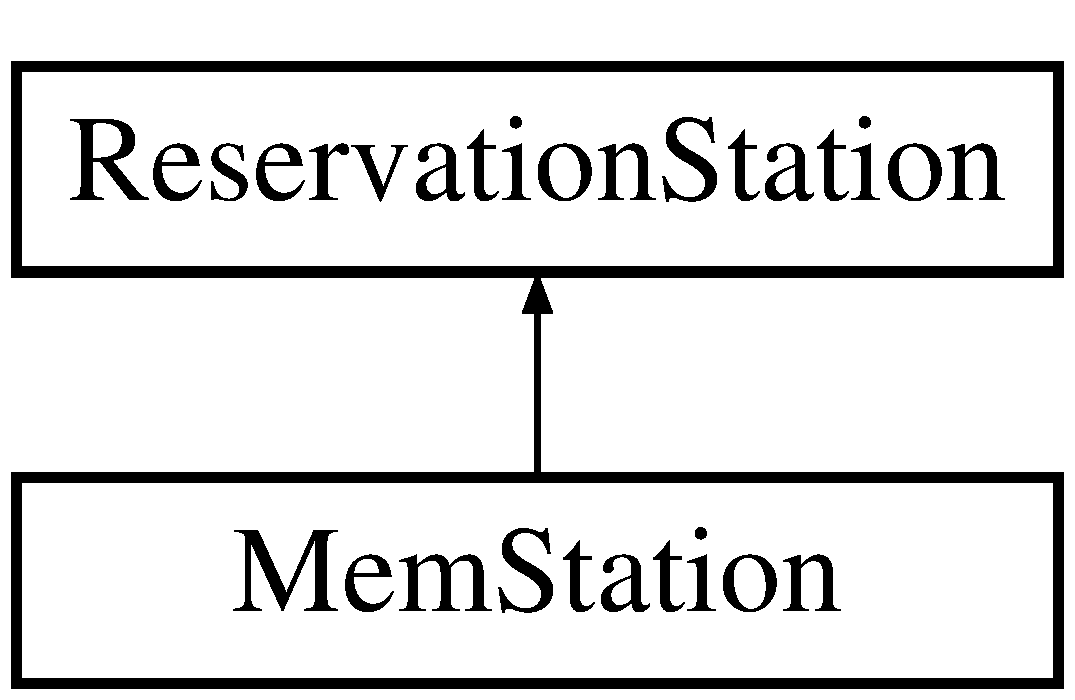
\includegraphics[height=2.000000cm]{classMemStation}
\end{center}
\end{figure}
\subsection*{\-Public \-Member \-Functions}
\begin{DoxyCompactItemize}
\item 
\hyperlink{classMemStation_a94ab3bf32e281cd07628b931b0a962f2}{\-Mem\-Station} (\-String \hyperlink{classReservationStation_a2c0bd5b95f126395b0ab081394f090f6}{sname})
\item 
void \hyperlink{classMemStation_ab02b57a1bea7277dab474c8ffd7ac5ac}{clear} ()
\item 
boolean \hyperlink{classMemStation_ac118dad2969d9bab0c2813b0e8681aa7}{is\-Ready} ()
\item 
\-String \hyperlink{classMemStation_a7488a8869905139d9a9ac0e0b7789327}{get\-Address} ()
\item 
void \hyperlink{classMemStation_a020c83f5370751b713b77bc5f419c06f}{set\-Address} (\-String \hyperlink{classMemStation_aeed8a623b07e146133976083b88ae513}{address})
\item 
boolean \hyperlink{classMemStation_a210ea0822fa342eae23ae190e38a0f96}{is\-Store} ()
\item 
void \hyperlink{classMemStation_af5cbfa20af449839121307147b3af436}{schedule\-Instruction} (\hyperlink{classOperation}{\-Operation} op, \hyperlink{classRegisterFiles}{\-Register\-Files} reg\-\_\-in, int cycles)
\item 
void \hyperlink{classMemStation_a4b9152fcfe59b601e7cf80e0a6ccc105}{update\-Addr\-Components} (\-String alias, \-String value)
\item 
boolean \hyperlink{classMemStation_afa9b7145ca1157b98d1f7d226b384b1d}{has\-Priority} (\-Hash\-Map$<$ \-String, \-Integer $>$ memory\-\_\-buffer)
\end{DoxyCompactItemize}
\subsection*{\-Static \-Public \-Member \-Functions}
\begin{DoxyCompactItemize}
\item 
static boolean \hyperlink{classMemStation_a75e3b4382aaa6cc851f89d7f9360dae3}{is\-Store} (\-String opcode)
\end{DoxyCompactItemize}
\subsection*{\-Private \-Member \-Functions}
\begin{DoxyCompactItemize}
\item 
void \hyperlink{classMemStation_a33eea591c23271c00768d3ec9b2eb92d}{update\-Address} ()
\item 
void \hyperlink{classMemStation_afe087bc173ab7dca0674621e42f36aa7}{set\-Store} ()
\end{DoxyCompactItemize}
\subsection*{\-Private \-Attributes}
\begin{DoxyCompactItemize}
\item 
\-String \hyperlink{classMemStation_aeed8a623b07e146133976083b88ae513}{address}
\begin{DoxyCompactList}\small\item\em \-Address to be stored or loaded from memory. \end{DoxyCompactList}\item 
\-String\mbox{[}$\,$\mbox{]} \hyperlink{classMemStation_a26f6ed03957088b12aec6200cf9ccd1e}{addr\-\_\-comp}
\begin{DoxyCompactList}\small\item\em \-Components used in computing the final address, and the register for stores \mbox{[}3\mbox{]}. \end{DoxyCompactList}\item 
boolean \hyperlink{classMemStation_acc8a77b7441e35271230350677d71b8f}{is\-\_\-store}
\begin{DoxyCompactList}\small\item\em \-True indicates that the current operation is a store. \end{DoxyCompactList}\end{DoxyCompactItemize}


\subsection{\-Detailed \-Description}
\-This class provides all \hyperlink{classMemStation}{\-Mem\-Station} functionality. 

\subsection{\-Constructor \& \-Destructor \-Documentation}
\hypertarget{classMemStation_a94ab3bf32e281cd07628b931b0a962f2}{\index{\-Mem\-Station@{\-Mem\-Station}!\-Mem\-Station@{\-Mem\-Station}}
\index{\-Mem\-Station@{\-Mem\-Station}!MemStation@{\-Mem\-Station}}
\subsubsection[{\-Mem\-Station}]{\setlength{\rightskip}{0pt plus 5cm}{\bf \-Mem\-Station.\-Mem\-Station} (
\begin{DoxyParamCaption}
\item[{\-String}]{sname}
\end{DoxyParamCaption}
)}}\label{classMemStation_a94ab3bf32e281cd07628b931b0a962f2}
\-Calls superclass constructor and initializes address 

\subsection{\-Member \-Function \-Documentation}
\hypertarget{classMemStation_ab02b57a1bea7277dab474c8ffd7ac5ac}{\index{\-Mem\-Station@{\-Mem\-Station}!clear@{clear}}
\index{clear@{clear}!MemStation@{\-Mem\-Station}}
\subsubsection[{clear}]{\setlength{\rightskip}{0pt plus 5cm}void {\bf \-Mem\-Station.\-clear} (
\begin{DoxyParamCaption}
{}
\end{DoxyParamCaption}
)\hspace{0.3cm}{\ttfamily  \mbox{[}virtual\mbox{]}}}}\label{classMemStation_ab02b57a1bea7277dab474c8ffd7ac5ac}
\-Function to clear the \-Reservation \-Station 

\-Implements \hyperlink{classReservationStation_a5788893e16b640dc7edbab832b1cb80d}{\-Reservation\-Station}.

\hypertarget{classMemStation_a7488a8869905139d9a9ac0e0b7789327}{\index{\-Mem\-Station@{\-Mem\-Station}!get\-Address@{get\-Address}}
\index{get\-Address@{get\-Address}!MemStation@{\-Mem\-Station}}
\subsubsection[{get\-Address}]{\setlength{\rightskip}{0pt plus 5cm}\-String {\bf \-Mem\-Station.\-get\-Address} (
\begin{DoxyParamCaption}
{}
\end{DoxyParamCaption}
)}}\label{classMemStation_a7488a8869905139d9a9ac0e0b7789327}
\-Function returns the value of address \hypertarget{classMemStation_afa9b7145ca1157b98d1f7d226b384b1d}{\index{\-Mem\-Station@{\-Mem\-Station}!has\-Priority@{has\-Priority}}
\index{has\-Priority@{has\-Priority}!MemStation@{\-Mem\-Station}}
\subsubsection[{has\-Priority}]{\setlength{\rightskip}{0pt plus 5cm}boolean {\bf \-Mem\-Station.\-has\-Priority} (
\begin{DoxyParamCaption}
\item[{\-Hash\-Map$<$ \-String, \-Integer $>$}]{memory\-\_\-buffer}
\end{DoxyParamCaption}
)}}\label{classMemStation_afa9b7145ca1157b98d1f7d226b384b1d}
\-Checks if the station has memory access priority \hypertarget{classMemStation_ac118dad2969d9bab0c2813b0e8681aa7}{\index{\-Mem\-Station@{\-Mem\-Station}!is\-Ready@{is\-Ready}}
\index{is\-Ready@{is\-Ready}!MemStation@{\-Mem\-Station}}
\subsubsection[{is\-Ready}]{\setlength{\rightskip}{0pt plus 5cm}boolean {\bf \-Mem\-Station.\-is\-Ready} (
\begin{DoxyParamCaption}
{}
\end{DoxyParamCaption}
)\hspace{0.3cm}{\ttfamily  \mbox{[}virtual\mbox{]}}}}\label{classMemStation_ac118dad2969d9bab0c2813b0e8681aa7}
\-Function to determine whether \hyperlink{classMemStation}{\-Mem\-Station} is \-Ready for use 

\-Implements \hyperlink{classReservationStation_a4fe26aca967123d4e9ec5aabf55d4d17}{\-Reservation\-Station}.

\hypertarget{classMemStation_a210ea0822fa342eae23ae190e38a0f96}{\index{\-Mem\-Station@{\-Mem\-Station}!is\-Store@{is\-Store}}
\index{is\-Store@{is\-Store}!MemStation@{\-Mem\-Station}}
\subsubsection[{is\-Store}]{\setlength{\rightskip}{0pt plus 5cm}boolean {\bf \-Mem\-Station.\-is\-Store} (
\begin{DoxyParamCaption}
{}
\end{DoxyParamCaption}
)}}\label{classMemStation_a210ea0822fa342eae23ae190e38a0f96}
\-Return whether the currently scheduled operation is a store \hypertarget{classMemStation_a75e3b4382aaa6cc851f89d7f9360dae3}{\index{\-Mem\-Station@{\-Mem\-Station}!is\-Store@{is\-Store}}
\index{is\-Store@{is\-Store}!MemStation@{\-Mem\-Station}}
\subsubsection[{is\-Store}]{\setlength{\rightskip}{0pt plus 5cm}static boolean {\bf \-Mem\-Station.\-is\-Store} (
\begin{DoxyParamCaption}
\item[{\-String}]{opcode}
\end{DoxyParamCaption}
)\hspace{0.3cm}{\ttfamily  \mbox{[}static\mbox{]}}}}\label{classMemStation_a75e3b4382aaa6cc851f89d7f9360dae3}
\-Static \-Function \-Classify the message as \-Store or \-Otther \hypertarget{classMemStation_af5cbfa20af449839121307147b3af436}{\index{\-Mem\-Station@{\-Mem\-Station}!schedule\-Instruction@{schedule\-Instruction}}
\index{schedule\-Instruction@{schedule\-Instruction}!MemStation@{\-Mem\-Station}}
\subsubsection[{schedule\-Instruction}]{\setlength{\rightskip}{0pt plus 5cm}void {\bf \-Mem\-Station.\-schedule\-Instruction} (
\begin{DoxyParamCaption}
\item[{{\bf \-Operation}}]{op, }
\item[{{\bf \-Register\-Files}}]{reg\-\_\-in, }
\item[{int}]{cycles}
\end{DoxyParamCaption}
)\hspace{0.3cm}{\ttfamily  \mbox{[}virtual\mbox{]}}}}\label{classMemStation_af5cbfa20af449839121307147b3af436}
\-Function to schedule the instruction 

\-Implements \hyperlink{classReservationStation_a5108e433a0a7e7cdd072fa7bcecdd399}{\-Reservation\-Station}.

\hypertarget{classMemStation_a020c83f5370751b713b77bc5f419c06f}{\index{\-Mem\-Station@{\-Mem\-Station}!set\-Address@{set\-Address}}
\index{set\-Address@{set\-Address}!MemStation@{\-Mem\-Station}}
\subsubsection[{set\-Address}]{\setlength{\rightskip}{0pt plus 5cm}void {\bf \-Mem\-Station.\-set\-Address} (
\begin{DoxyParamCaption}
\item[{\-String}]{address}
\end{DoxyParamCaption}
)}}\label{classMemStation_a020c83f5370751b713b77bc5f419c06f}
\-Function sets the value of address \hypertarget{classMemStation_afe087bc173ab7dca0674621e42f36aa7}{\index{\-Mem\-Station@{\-Mem\-Station}!set\-Store@{set\-Store}}
\index{set\-Store@{set\-Store}!MemStation@{\-Mem\-Station}}
\subsubsection[{set\-Store}]{\setlength{\rightskip}{0pt plus 5cm}void {\bf \-Mem\-Station.\-set\-Store} (
\begin{DoxyParamCaption}
{}
\end{DoxyParamCaption}
)\hspace{0.3cm}{\ttfamily  \mbox{[}private\mbox{]}}}}\label{classMemStation_afe087bc173ab7dca0674621e42f36aa7}
\-Utility funtion to set the message as load or store \hypertarget{classMemStation_a4b9152fcfe59b601e7cf80e0a6ccc105}{\index{\-Mem\-Station@{\-Mem\-Station}!update\-Addr\-Components@{update\-Addr\-Components}}
\index{update\-Addr\-Components@{update\-Addr\-Components}!MemStation@{\-Mem\-Station}}
\subsubsection[{update\-Addr\-Components}]{\setlength{\rightskip}{0pt plus 5cm}void {\bf \-Mem\-Station.\-update\-Addr\-Components} (
\begin{DoxyParamCaption}
\item[{\-String}]{alias, }
\item[{\-String}]{value}
\end{DoxyParamCaption}
)}}\label{classMemStation_a4b9152fcfe59b601e7cf80e0a6ccc105}
\-Update the address components \hypertarget{classMemStation_a33eea591c23271c00768d3ec9b2eb92d}{\index{\-Mem\-Station@{\-Mem\-Station}!update\-Address@{update\-Address}}
\index{update\-Address@{update\-Address}!MemStation@{\-Mem\-Station}}
\subsubsection[{update\-Address}]{\setlength{\rightskip}{0pt plus 5cm}void {\bf \-Mem\-Station.\-update\-Address} (
\begin{DoxyParamCaption}
{}
\end{DoxyParamCaption}
)\hspace{0.3cm}{\ttfamily  \mbox{[}private\mbox{]}}}}\label{classMemStation_a33eea591c23271c00768d3ec9b2eb92d}
\-Utility function to update the address 

\subsection{\-Member \-Data \-Documentation}
\hypertarget{classMemStation_a26f6ed03957088b12aec6200cf9ccd1e}{\index{\-Mem\-Station@{\-Mem\-Station}!addr\-\_\-comp@{addr\-\_\-comp}}
\index{addr\-\_\-comp@{addr\-\_\-comp}!MemStation@{\-Mem\-Station}}
\subsubsection[{addr\-\_\-comp}]{\setlength{\rightskip}{0pt plus 5cm}\-String \mbox{[}$\,$\mbox{]} {\bf \-Mem\-Station.\-addr\-\_\-comp}\hspace{0.3cm}{\ttfamily  \mbox{[}private\mbox{]}}}}\label{classMemStation_a26f6ed03957088b12aec6200cf9ccd1e}


\-Components used in computing the final address, and the register for stores \mbox{[}3\mbox{]}. 

\hypertarget{classMemStation_aeed8a623b07e146133976083b88ae513}{\index{\-Mem\-Station@{\-Mem\-Station}!address@{address}}
\index{address@{address}!MemStation@{\-Mem\-Station}}
\subsubsection[{address}]{\setlength{\rightskip}{0pt plus 5cm}\-String {\bf \-Mem\-Station.\-address}\hspace{0.3cm}{\ttfamily  \mbox{[}private\mbox{]}}}}\label{classMemStation_aeed8a623b07e146133976083b88ae513}


\-Address to be stored or loaded from memory. 

\hypertarget{classMemStation_acc8a77b7441e35271230350677d71b8f}{\index{\-Mem\-Station@{\-Mem\-Station}!is\-\_\-store@{is\-\_\-store}}
\index{is\-\_\-store@{is\-\_\-store}!MemStation@{\-Mem\-Station}}
\subsubsection[{is\-\_\-store}]{\setlength{\rightskip}{0pt plus 5cm}boolean {\bf \-Mem\-Station.\-is\-\_\-store}\hspace{0.3cm}{\ttfamily  \mbox{[}private\mbox{]}}}}\label{classMemStation_acc8a77b7441e35271230350677d71b8f}


\-True indicates that the current operation is a store. 



\-The documentation for this class was generated from the following file\-:\begin{DoxyCompactItemize}
\item 
\hyperlink{MemStation_8java}{\-Mem\-Station.\-java}\end{DoxyCompactItemize}

\hypertarget{classOperation}{\section{\-Operation \-Class \-Reference}
\label{classOperation}\index{\-Operation@{\-Operation}}
}
\subsection*{\-Public \-Member \-Functions}
\begin{DoxyCompactItemize}
\item 
\hyperlink{classOperation_a91e0f1079df0a9ce564816aa610a5335}{\-Operation} ()
\item 
\hyperlink{classOperation_a2e21fd9203d0f82233a25c0930a64fff}{\-Operation} (\-String \hyperlink{classOperation_a91a69611ab1dd4ca12de1abdd49c2b42}{opcode}, \-String operand\-\_\-1, \-String operand\-\_\-2, \-String operand\-\_\-3, boolean \hyperlink{classOperation_ac3f08d5e96c77223a1fbfa68afb0d63a}{has\-\_\-comment})
\item 
\hyperlink{classOperation_a5b9b14110e36a150abba066a98c96e81}{\-Operation} (\-String \hyperlink{classOperation_a91a69611ab1dd4ca12de1abdd49c2b42}{opcode}, \-String operand\-\_\-1, \-String operand\-\_\-2, boolean \hyperlink{classOperation_ac3f08d5e96c77223a1fbfa68afb0d63a}{has\-\_\-comment})
\item 
\hyperlink{classOperation_ad4446a177e8fee8190c847711dd040e3}{\-Operation} (\hyperlink{classOperation}{\-Operation} to\-\_\-copy)
\item 
boolean \hyperlink{classOperation_aa2db062dbc961ac619c3fdf87409b2f1}{has\-Comment} ()
\item 
\-String \hyperlink{classOperation_a1fee9b845f368eaa45f8c3a59fdc6768}{get\-Opcode} ()
\item 
\-String \hyperlink{classOperation_aa1f781d95004579b19a32edd7cf13b53}{get\-Comment} ()
\item 
\-String \hyperlink{classOperation_a532c5b1c649dfa9864279f545f5e0b8d}{get\-Operand} (int number)
\item 
int \hyperlink{classOperation_a96f020f9945950f2f753f7d1a0aa988b}{get\-Number\-Of\-Operands} ()
\item 
\-String \hyperlink{classOperation_a1e310aee2b5aeefa8094d2197816af9b}{get\-Operands} ()
\item 
int \hyperlink{classOperation_a840cc134fbf5b2374b2b427a754fb4bf}{get\-Exec\-Start} ()
\item 
int \hyperlink{classOperation_a75c1ec9890127365d2b646d0a725a3bd}{get\-Exec\-End} ()
\item 
int \hyperlink{classOperation_a5accacc3ce8e2653bd3b65ddef058670}{get\-Issue\-Num} ()
\item 
\-String \hyperlink{classOperation_aabe96409ea6c517e07c07277a9bd6be6}{get\-Execution} ()
\item 
int \hyperlink{classOperation_ad8b1f145050d381688535a3311d48143}{get\-Write\-Time} ()
\item 
void \hyperlink{classOperation_ac8493946ebb2ff362b7a9826c515aef4}{set\-Opcode} (\-String \hyperlink{classOperation_a91a69611ab1dd4ca12de1abdd49c2b42}{opcode})
\item 
void \hyperlink{classOperation_a4bb7b2db5560ac84940f305207b31404}{set\-Comment} (\-String \hyperlink{classOperation_a3b56588030b54deb7ffb0c5f0a4ebe68}{comment})
\item 
void \hyperlink{classOperation_af84aceab243ad1c694e749b83a233d1a}{set\-Operand} (int number, \-String operand\-\_\-in)  throws Exception
\item 
void \hyperlink{classOperation_a47af41a9f8ee13b0038fe6de3c96c804}{set\-Exec\-Start} (int n)
\item 
void \hyperlink{classOperation_ac0b7d71ca5cc03ed25fa7c069b6c4ea1}{set\-Exec\-End} (int n)
\item 
void \hyperlink{classOperation_ab5c62892336b30cec49b36dd01503def}{set\-Write\-Time} (int n)
\item 
void \hyperlink{classOperation_a333309bc371302cdbfab142cd9775032}{set\-Issue\-Num} (int i)
\item 
\-String \hyperlink{classOperation_a14f47977fe6f954977bbe1fc558c7174}{to\-String} ()
\end{DoxyCompactItemize}
\subsection*{\-Package \-Functions}
\begin{DoxyCompactItemize}
\item 
boolean \hyperlink{classOperation_a78754fb1285604d5802ecd482386eb24}{is\-Scheduled} ()
\item 
void \hyperlink{classOperation_a8267763b76c5e32c4cc748db3d2df27e}{set\-Scheduled} ()
\end{DoxyCompactItemize}
\subsection*{\-Package \-Attributes}
\begin{DoxyCompactItemize}
\item 
int \hyperlink{classOperation_aaea255d6ed7bf51b531179aa87cb5b6d}{exec\-\_\-end}
\begin{DoxyCompactList}\small\item\em start and end of executions respectively \end{DoxyCompactList}\end{DoxyCompactItemize}
\subsection*{\-Private \-Attributes}
\begin{DoxyCompactItemize}
\item 
\-String \hyperlink{classOperation_a91a69611ab1dd4ca12de1abdd49c2b42}{opcode}
\begin{DoxyCompactList}\small\item\em \-Contains the opcode. \end{DoxyCompactList}\item 
\-String \hyperlink{classOperation_a3b56588030b54deb7ffb0c5f0a4ebe68}{comment}
\begin{DoxyCompactList}\small\item\em \-Stores the comment. \end{DoxyCompactList}\item 
\-String\mbox{[}$\,$\mbox{]} \hyperlink{classOperation_ae5923860533d63c6a35d658b2683a994}{operands}
\begin{DoxyCompactList}\small\item\em \-Stores all operands. \end{DoxyCompactList}\item 
int \hyperlink{classOperation_a2dfe9cb6c6a10cb7f775036b6602bf7e}{exec\-\_\-start}
\item 
int \hyperlink{classOperation_a53e016dd4e33bdb373ca7d09d5cb8e83}{time\-\_\-write}
\begin{DoxyCompactList}\small\item\em \-Write time. \end{DoxyCompactList}\item 
int \hyperlink{classOperation_af9f72f137e8122fecde6cb26ea01db5d}{issue}
\begin{DoxyCompactList}\small\item\em issue number \end{DoxyCompactList}\item 
boolean \hyperlink{classOperation_ac3f08d5e96c77223a1fbfa68afb0d63a}{has\-\_\-comment}
\begin{DoxyCompactList}\small\item\em \-Specifies the existance of a comment. \end{DoxyCompactList}\item 
boolean \hyperlink{classOperation_a1455e6e40b057e3f25e29f7a54c6920f}{scheduled}
\begin{DoxyCompactList}\small\item\em \-Set to true when the instruction has been scheduled. \end{DoxyCompactList}\end{DoxyCompactItemize}


\subsection{\-Detailed \-Description}
\-This class provides all \hyperlink{classOperation}{\-Operation} functionality. 

\subsection{\-Constructor \& \-Destructor \-Documentation}
\hypertarget{classOperation_a91e0f1079df0a9ce564816aa610a5335}{\index{\-Operation@{\-Operation}!\-Operation@{\-Operation}}
\index{\-Operation@{\-Operation}!Operation@{\-Operation}}
\subsubsection[{\-Operation}]{\setlength{\rightskip}{0pt plus 5cm}{\bf \-Operation.\-Operation} (
\begin{DoxyParamCaption}
{}
\end{DoxyParamCaption}
)}}\label{classOperation_a91e0f1079df0a9ce564816aa610a5335}
\hypertarget{classOperation_a2e21fd9203d0f82233a25c0930a64fff}{\index{\-Operation@{\-Operation}!\-Operation@{\-Operation}}
\index{\-Operation@{\-Operation}!Operation@{\-Operation}}
\subsubsection[{\-Operation}]{\setlength{\rightskip}{0pt plus 5cm}{\bf \-Operation.\-Operation} (
\begin{DoxyParamCaption}
\item[{\-String}]{opcode, }
\item[{\-String}]{operand\-\_\-1, }
\item[{\-String}]{operand\-\_\-2, }
\item[{\-String}]{operand\-\_\-3, }
\item[{boolean}]{has\-\_\-comment}
\end{DoxyParamCaption}
)}}\label{classOperation_a2e21fd9203d0f82233a25c0930a64fff}
\-Construct an \hyperlink{classOperation}{\-Operation} object give 1 opcode, 3 operands and a boolean. \hypertarget{classOperation_a5b9b14110e36a150abba066a98c96e81}{\index{\-Operation@{\-Operation}!\-Operation@{\-Operation}}
\index{\-Operation@{\-Operation}!Operation@{\-Operation}}
\subsubsection[{\-Operation}]{\setlength{\rightskip}{0pt plus 5cm}{\bf \-Operation.\-Operation} (
\begin{DoxyParamCaption}
\item[{\-String}]{opcode, }
\item[{\-String}]{operand\-\_\-1, }
\item[{\-String}]{operand\-\_\-2, }
\item[{boolean}]{has\-\_\-comment}
\end{DoxyParamCaption}
)}}\label{classOperation_a5b9b14110e36a150abba066a98c96e81}
\-Construct an \hyperlink{classOperation}{\-Operation} object give 1 opcode, 2 operands and a boolean. \hypertarget{classOperation_ad4446a177e8fee8190c847711dd040e3}{\index{\-Operation@{\-Operation}!\-Operation@{\-Operation}}
\index{\-Operation@{\-Operation}!Operation@{\-Operation}}
\subsubsection[{\-Operation}]{\setlength{\rightskip}{0pt plus 5cm}{\bf \-Operation.\-Operation} (
\begin{DoxyParamCaption}
\item[{{\bf \-Operation}}]{to\-\_\-copy}
\end{DoxyParamCaption}
)}}\label{classOperation_ad4446a177e8fee8190c847711dd040e3}
\-Construct an \hyperlink{classOperation}{\-Operation} object given an existing \hyperlink{classOperation}{\-Operation} object. 

\subsection{\-Member \-Function \-Documentation}
\hypertarget{classOperation_aa1f781d95004579b19a32edd7cf13b53}{\index{\-Operation@{\-Operation}!get\-Comment@{get\-Comment}}
\index{get\-Comment@{get\-Comment}!Operation@{\-Operation}}
\subsubsection[{get\-Comment}]{\setlength{\rightskip}{0pt plus 5cm}\-String {\bf \-Operation.\-get\-Comment} (
\begin{DoxyParamCaption}
{}
\end{DoxyParamCaption}
)}}\label{classOperation_aa1f781d95004579b19a32edd7cf13b53}
\-Return the comment. \hypertarget{classOperation_a75c1ec9890127365d2b646d0a725a3bd}{\index{\-Operation@{\-Operation}!get\-Exec\-End@{get\-Exec\-End}}
\index{get\-Exec\-End@{get\-Exec\-End}!Operation@{\-Operation}}
\subsubsection[{get\-Exec\-End}]{\setlength{\rightskip}{0pt plus 5cm}int {\bf \-Operation.\-get\-Exec\-End} (
\begin{DoxyParamCaption}
{}
\end{DoxyParamCaption}
)}}\label{classOperation_a75c1ec9890127365d2b646d0a725a3bd}
\-Get execution end \hypertarget{classOperation_a840cc134fbf5b2374b2b427a754fb4bf}{\index{\-Operation@{\-Operation}!get\-Exec\-Start@{get\-Exec\-Start}}
\index{get\-Exec\-Start@{get\-Exec\-Start}!Operation@{\-Operation}}
\subsubsection[{get\-Exec\-Start}]{\setlength{\rightskip}{0pt plus 5cm}int {\bf \-Operation.\-get\-Exec\-Start} (
\begin{DoxyParamCaption}
{}
\end{DoxyParamCaption}
)}}\label{classOperation_a840cc134fbf5b2374b2b427a754fb4bf}
\-Get execution start \hypertarget{classOperation_aabe96409ea6c517e07c07277a9bd6be6}{\index{\-Operation@{\-Operation}!get\-Execution@{get\-Execution}}
\index{get\-Execution@{get\-Execution}!Operation@{\-Operation}}
\subsubsection[{get\-Execution}]{\setlength{\rightskip}{0pt plus 5cm}\-String {\bf \-Operation.\-get\-Execution} (
\begin{DoxyParamCaption}
{}
\end{DoxyParamCaption}
)}}\label{classOperation_aabe96409ea6c517e07c07277a9bd6be6}
\-Get execution description \hypertarget{classOperation_a5accacc3ce8e2653bd3b65ddef058670}{\index{\-Operation@{\-Operation}!get\-Issue\-Num@{get\-Issue\-Num}}
\index{get\-Issue\-Num@{get\-Issue\-Num}!Operation@{\-Operation}}
\subsubsection[{get\-Issue\-Num}]{\setlength{\rightskip}{0pt plus 5cm}int {\bf \-Operation.\-get\-Issue\-Num} (
\begin{DoxyParamCaption}
{}
\end{DoxyParamCaption}
)}}\label{classOperation_a5accacc3ce8e2653bd3b65ddef058670}
\-Get the issue number \hypertarget{classOperation_a96f020f9945950f2f753f7d1a0aa988b}{\index{\-Operation@{\-Operation}!get\-Number\-Of\-Operands@{get\-Number\-Of\-Operands}}
\index{get\-Number\-Of\-Operands@{get\-Number\-Of\-Operands}!Operation@{\-Operation}}
\subsubsection[{get\-Number\-Of\-Operands}]{\setlength{\rightskip}{0pt plus 5cm}int {\bf \-Operation.\-get\-Number\-Of\-Operands} (
\begin{DoxyParamCaption}
{}
\end{DoxyParamCaption}
)}}\label{classOperation_a96f020f9945950f2f753f7d1a0aa988b}
\-Return the number of operands \hypertarget{classOperation_a1fee9b845f368eaa45f8c3a59fdc6768}{\index{\-Operation@{\-Operation}!get\-Opcode@{get\-Opcode}}
\index{get\-Opcode@{get\-Opcode}!Operation@{\-Operation}}
\subsubsection[{get\-Opcode}]{\setlength{\rightskip}{0pt plus 5cm}\-String {\bf \-Operation.\-get\-Opcode} (
\begin{DoxyParamCaption}
{}
\end{DoxyParamCaption}
)}}\label{classOperation_a1fee9b845f368eaa45f8c3a59fdc6768}
\-Return the opcode -\/-\/ exempli gratia \-L\-O\-A\-D, \-S\-D, \-D\-A\-D\-D\-I. \hypertarget{classOperation_a532c5b1c649dfa9864279f545f5e0b8d}{\index{\-Operation@{\-Operation}!get\-Operand@{get\-Operand}}
\index{get\-Operand@{get\-Operand}!Operation@{\-Operation}}
\subsubsection[{get\-Operand}]{\setlength{\rightskip}{0pt plus 5cm}\-String {\bf \-Operation.\-get\-Operand} (
\begin{DoxyParamCaption}
\item[{int}]{number}
\end{DoxyParamCaption}
)}}\label{classOperation_a532c5b1c649dfa9864279f545f5e0b8d}
\-Get the operand at the specified position. \-Positions start at \char`\"{}1\char`\"{}. \hypertarget{classOperation_a1e310aee2b5aeefa8094d2197816af9b}{\index{\-Operation@{\-Operation}!get\-Operands@{get\-Operands}}
\index{get\-Operands@{get\-Operands}!Operation@{\-Operation}}
\subsubsection[{get\-Operands}]{\setlength{\rightskip}{0pt plus 5cm}\-String {\bf \-Operation.\-get\-Operands} (
\begin{DoxyParamCaption}
{}
\end{DoxyParamCaption}
)}}\label{classOperation_a1e310aee2b5aeefa8094d2197816af9b}
\-Return a \-String containing all operands. \hypertarget{classOperation_ad8b1f145050d381688535a3311d48143}{\index{\-Operation@{\-Operation}!get\-Write\-Time@{get\-Write\-Time}}
\index{get\-Write\-Time@{get\-Write\-Time}!Operation@{\-Operation}}
\subsubsection[{get\-Write\-Time}]{\setlength{\rightskip}{0pt plus 5cm}int {\bf \-Operation.\-get\-Write\-Time} (
\begin{DoxyParamCaption}
{}
\end{DoxyParamCaption}
)}}\label{classOperation_ad8b1f145050d381688535a3311d48143}
\-Get the time the result was written \hypertarget{classOperation_aa2db062dbc961ac619c3fdf87409b2f1}{\index{\-Operation@{\-Operation}!has\-Comment@{has\-Comment}}
\index{has\-Comment@{has\-Comment}!Operation@{\-Operation}}
\subsubsection[{has\-Comment}]{\setlength{\rightskip}{0pt plus 5cm}boolean {\bf \-Operation.\-has\-Comment} (
\begin{DoxyParamCaption}
{}
\end{DoxyParamCaption}
)}}\label{classOperation_aa2db062dbc961ac619c3fdf87409b2f1}
\-Return whether a comment exists \hypertarget{classOperation_a78754fb1285604d5802ecd482386eb24}{\index{\-Operation@{\-Operation}!is\-Scheduled@{is\-Scheduled}}
\index{is\-Scheduled@{is\-Scheduled}!Operation@{\-Operation}}
\subsubsection[{is\-Scheduled}]{\setlength{\rightskip}{0pt plus 5cm}boolean {\bf \-Operation.\-is\-Scheduled} (
\begin{DoxyParamCaption}
{}
\end{DoxyParamCaption}
)\hspace{0.3cm}{\ttfamily  \mbox{[}package\mbox{]}}}}\label{classOperation_a78754fb1285604d5802ecd482386eb24}
\-Return whether the instruction has been scheduled \hypertarget{classOperation_a4bb7b2db5560ac84940f305207b31404}{\index{\-Operation@{\-Operation}!set\-Comment@{set\-Comment}}
\index{set\-Comment@{set\-Comment}!Operation@{\-Operation}}
\subsubsection[{set\-Comment}]{\setlength{\rightskip}{0pt plus 5cm}void {\bf \-Operation.\-set\-Comment} (
\begin{DoxyParamCaption}
\item[{\-String}]{comment}
\end{DoxyParamCaption}
)}}\label{classOperation_a4bb7b2db5560ac84940f305207b31404}
\-Set a comment \hypertarget{classOperation_ac0b7d71ca5cc03ed25fa7c069b6c4ea1}{\index{\-Operation@{\-Operation}!set\-Exec\-End@{set\-Exec\-End}}
\index{set\-Exec\-End@{set\-Exec\-End}!Operation@{\-Operation}}
\subsubsection[{set\-Exec\-End}]{\setlength{\rightskip}{0pt plus 5cm}void {\bf \-Operation.\-set\-Exec\-End} (
\begin{DoxyParamCaption}
\item[{int}]{n}
\end{DoxyParamCaption}
)}}\label{classOperation_ac0b7d71ca5cc03ed25fa7c069b6c4ea1}
\-Set execution end \hypertarget{classOperation_a47af41a9f8ee13b0038fe6de3c96c804}{\index{\-Operation@{\-Operation}!set\-Exec\-Start@{set\-Exec\-Start}}
\index{set\-Exec\-Start@{set\-Exec\-Start}!Operation@{\-Operation}}
\subsubsection[{set\-Exec\-Start}]{\setlength{\rightskip}{0pt plus 5cm}void {\bf \-Operation.\-set\-Exec\-Start} (
\begin{DoxyParamCaption}
\item[{int}]{n}
\end{DoxyParamCaption}
)}}\label{classOperation_a47af41a9f8ee13b0038fe6de3c96c804}
\-Set execution start \hypertarget{classOperation_a333309bc371302cdbfab142cd9775032}{\index{\-Operation@{\-Operation}!set\-Issue\-Num@{set\-Issue\-Num}}
\index{set\-Issue\-Num@{set\-Issue\-Num}!Operation@{\-Operation}}
\subsubsection[{set\-Issue\-Num}]{\setlength{\rightskip}{0pt plus 5cm}void {\bf \-Operation.\-set\-Issue\-Num} (
\begin{DoxyParamCaption}
\item[{int}]{i}
\end{DoxyParamCaption}
)}}\label{classOperation_a333309bc371302cdbfab142cd9775032}
\-Set the issue number \hypertarget{classOperation_ac8493946ebb2ff362b7a9826c515aef4}{\index{\-Operation@{\-Operation}!set\-Opcode@{set\-Opcode}}
\index{set\-Opcode@{set\-Opcode}!Operation@{\-Operation}}
\subsubsection[{set\-Opcode}]{\setlength{\rightskip}{0pt plus 5cm}void {\bf \-Operation.\-set\-Opcode} (
\begin{DoxyParamCaption}
\item[{\-String}]{opcode}
\end{DoxyParamCaption}
)}}\label{classOperation_ac8493946ebb2ff362b7a9826c515aef4}
\-Set the \hyperlink{classOperation}{\-Operation} opcode. \hypertarget{classOperation_af84aceab243ad1c694e749b83a233d1a}{\index{\-Operation@{\-Operation}!set\-Operand@{set\-Operand}}
\index{set\-Operand@{set\-Operand}!Operation@{\-Operation}}
\subsubsection[{set\-Operand}]{\setlength{\rightskip}{0pt plus 5cm}void {\bf \-Operation.\-set\-Operand} (
\begin{DoxyParamCaption}
\item[{int}]{number, }
\item[{\-String}]{operand\-\_\-in}
\end{DoxyParamCaption}
)  throws \-Exception}}\label{classOperation_af84aceab243ad1c694e749b83a233d1a}
\-Set the operand at the specified position. \-Positions start at \char`\"{}1\char`\"{}. \-Return an error if the position is invalid. \hypertarget{classOperation_a8267763b76c5e32c4cc748db3d2df27e}{\index{\-Operation@{\-Operation}!set\-Scheduled@{set\-Scheduled}}
\index{set\-Scheduled@{set\-Scheduled}!Operation@{\-Operation}}
\subsubsection[{set\-Scheduled}]{\setlength{\rightskip}{0pt plus 5cm}void {\bf \-Operation.\-set\-Scheduled} (
\begin{DoxyParamCaption}
{}
\end{DoxyParamCaption}
)\hspace{0.3cm}{\ttfamily  \mbox{[}package\mbox{]}}}}\label{classOperation_a8267763b76c5e32c4cc748db3d2df27e}
\-Set the scheduled flag \hypertarget{classOperation_ab5c62892336b30cec49b36dd01503def}{\index{\-Operation@{\-Operation}!set\-Write\-Time@{set\-Write\-Time}}
\index{set\-Write\-Time@{set\-Write\-Time}!Operation@{\-Operation}}
\subsubsection[{set\-Write\-Time}]{\setlength{\rightskip}{0pt plus 5cm}void {\bf \-Operation.\-set\-Write\-Time} (
\begin{DoxyParamCaption}
\item[{int}]{n}
\end{DoxyParamCaption}
)}}\label{classOperation_ab5c62892336b30cec49b36dd01503def}
\-Set the time the result was written \hypertarget{classOperation_a14f47977fe6f954977bbe1fc558c7174}{\index{\-Operation@{\-Operation}!to\-String@{to\-String}}
\index{to\-String@{to\-String}!Operation@{\-Operation}}
\subsubsection[{to\-String}]{\setlength{\rightskip}{0pt plus 5cm}\-String {\bf \-Operation.\-to\-String} (
\begin{DoxyParamCaption}
{}
\end{DoxyParamCaption}
)}}\label{classOperation_a14f47977fe6f954977bbe1fc558c7174}
\-Return the string represeation of the \hyperlink{classOperation}{\-Operation} object. 

\subsection{\-Member \-Data \-Documentation}
\hypertarget{classOperation_a3b56588030b54deb7ffb0c5f0a4ebe68}{\index{\-Operation@{\-Operation}!comment@{comment}}
\index{comment@{comment}!Operation@{\-Operation}}
\subsubsection[{comment}]{\setlength{\rightskip}{0pt plus 5cm}\-String {\bf \-Operation.\-comment}\hspace{0.3cm}{\ttfamily  \mbox{[}private\mbox{]}}}}\label{classOperation_a3b56588030b54deb7ffb0c5f0a4ebe68}


\-Stores the comment. 

\hypertarget{classOperation_aaea255d6ed7bf51b531179aa87cb5b6d}{\index{\-Operation@{\-Operation}!exec\-\_\-end@{exec\-\_\-end}}
\index{exec\-\_\-end@{exec\-\_\-end}!Operation@{\-Operation}}
\subsubsection[{exec\-\_\-end}]{\setlength{\rightskip}{0pt plus 5cm}int {\bf \-Operation.\-exec\-\_\-end}\hspace{0.3cm}{\ttfamily  \mbox{[}package\mbox{]}}}}\label{classOperation_aaea255d6ed7bf51b531179aa87cb5b6d}


start and end of executions respectively 

\hypertarget{classOperation_a2dfe9cb6c6a10cb7f775036b6602bf7e}{\index{\-Operation@{\-Operation}!exec\-\_\-start@{exec\-\_\-start}}
\index{exec\-\_\-start@{exec\-\_\-start}!Operation@{\-Operation}}
\subsubsection[{exec\-\_\-start}]{\setlength{\rightskip}{0pt plus 5cm}int {\bf \-Operation.\-exec\-\_\-start}\hspace{0.3cm}{\ttfamily  \mbox{[}private\mbox{]}}}}\label{classOperation_a2dfe9cb6c6a10cb7f775036b6602bf7e}
\hypertarget{classOperation_ac3f08d5e96c77223a1fbfa68afb0d63a}{\index{\-Operation@{\-Operation}!has\-\_\-comment@{has\-\_\-comment}}
\index{has\-\_\-comment@{has\-\_\-comment}!Operation@{\-Operation}}
\subsubsection[{has\-\_\-comment}]{\setlength{\rightskip}{0pt plus 5cm}boolean {\bf \-Operation.\-has\-\_\-comment}\hspace{0.3cm}{\ttfamily  \mbox{[}private\mbox{]}}}}\label{classOperation_ac3f08d5e96c77223a1fbfa68afb0d63a}


\-Specifies the existance of a comment. 

\hypertarget{classOperation_af9f72f137e8122fecde6cb26ea01db5d}{\index{\-Operation@{\-Operation}!issue@{issue}}
\index{issue@{issue}!Operation@{\-Operation}}
\subsubsection[{issue}]{\setlength{\rightskip}{0pt plus 5cm}int {\bf \-Operation.\-issue}\hspace{0.3cm}{\ttfamily  \mbox{[}private\mbox{]}}}}\label{classOperation_af9f72f137e8122fecde6cb26ea01db5d}


issue number 

\hypertarget{classOperation_a91a69611ab1dd4ca12de1abdd49c2b42}{\index{\-Operation@{\-Operation}!opcode@{opcode}}
\index{opcode@{opcode}!Operation@{\-Operation}}
\subsubsection[{opcode}]{\setlength{\rightskip}{0pt plus 5cm}\-String {\bf \-Operation.\-opcode}\hspace{0.3cm}{\ttfamily  \mbox{[}private\mbox{]}}}}\label{classOperation_a91a69611ab1dd4ca12de1abdd49c2b42}


\-Contains the opcode. 

\hypertarget{classOperation_ae5923860533d63c6a35d658b2683a994}{\index{\-Operation@{\-Operation}!operands@{operands}}
\index{operands@{operands}!Operation@{\-Operation}}
\subsubsection[{operands}]{\setlength{\rightskip}{0pt plus 5cm}\-String \mbox{[}$\,$\mbox{]} {\bf \-Operation.\-operands}\hspace{0.3cm}{\ttfamily  \mbox{[}private\mbox{]}}}}\label{classOperation_ae5923860533d63c6a35d658b2683a994}


\-Stores all operands. 

\hypertarget{classOperation_a1455e6e40b057e3f25e29f7a54c6920f}{\index{\-Operation@{\-Operation}!scheduled@{scheduled}}
\index{scheduled@{scheduled}!Operation@{\-Operation}}
\subsubsection[{scheduled}]{\setlength{\rightskip}{0pt plus 5cm}boolean {\bf \-Operation.\-scheduled}\hspace{0.3cm}{\ttfamily  \mbox{[}private\mbox{]}}}}\label{classOperation_a1455e6e40b057e3f25e29f7a54c6920f}


\-Set to true when the instruction has been scheduled. 

\hypertarget{classOperation_a53e016dd4e33bdb373ca7d09d5cb8e83}{\index{\-Operation@{\-Operation}!time\-\_\-write@{time\-\_\-write}}
\index{time\-\_\-write@{time\-\_\-write}!Operation@{\-Operation}}
\subsubsection[{time\-\_\-write}]{\setlength{\rightskip}{0pt plus 5cm}int {\bf \-Operation.\-time\-\_\-write}\hspace{0.3cm}{\ttfamily  \mbox{[}private\mbox{]}}}}\label{classOperation_a53e016dd4e33bdb373ca7d09d5cb8e83}


\-Write time. 



\-The documentation for this class was generated from the following file\-:\begin{DoxyCompactItemize}
\item 
\hyperlink{Operation_8java}{\-Operation.\-java}\end{DoxyCompactItemize}

\hypertarget{classOperationFileParser}{
\section{OperationFileParser Class Reference}
\label{classOperationFileParser}\index{OperationFileParser@{OperationFileParser}}
}
\subsection*{Public Member Functions}
\begin{DoxyCompactItemize}
\item 
\hyperlink{classOperationFileParser_aae642f641952d9299ae1d18c2a98e257}{OperationFileParser} ()
\item 
\hyperlink{classOperationFileParser_ab3cf3d1b41d42f6ce2a843fbe11a5f9a}{OperationFileParser} (String \hyperlink{classOperationFileParser_a02c7ed52d4be7f9a23054eebcff0a96e}{filename})
\item 
void \hyperlink{classOperationFileParser_af360317f51081606c8fb05b658be8d00}{parseFile} (\hyperlink{classOperationList}{OperationList} oplist, \hyperlink{classRegisterFiles}{RegisterFiles} reg\_\-files)  throws Exception
\item 
String \hyperlink{classOperationFileParser_af6e91ca0ed2166c6b75ad12574dc5341}{toString} ()
\end{DoxyCompactItemize}
\subsection*{Private Attributes}
\begin{DoxyCompactItemize}
\item 
String \hyperlink{classOperationFileParser_a02c7ed52d4be7f9a23054eebcff0a96e}{filename}
\begin{DoxyCompactList}\small\item\em The input filename. \item\end{DoxyCompactList}\end{DoxyCompactItemize}


\subsection{Detailed Description}
This class provides all file parsing funtionality. Given an input file, one \hyperlink{classOperationList}{OperationList} and one \hyperlink{classRegisterFiles}{RegisterFiles} will be generated. 

\subsection{Constructor \& Destructor Documentation}
\hypertarget{classOperationFileParser_aae642f641952d9299ae1d18c2a98e257}{
\index{OperationFileParser@{OperationFileParser}!OperationFileParser@{OperationFileParser}}
\index{OperationFileParser@{OperationFileParser}!OperationFileParser@{OperationFileParser}}
\subsubsection[{OperationFileParser}]{\setlength{\rightskip}{0pt plus 5cm}OperationFileParser.OperationFileParser (
\begin{DoxyParamCaption}
{}
\end{DoxyParamCaption}
)}}
\label{classOperationFileParser_aae642f641952d9299ae1d18c2a98e257}
Set the input file to the default value of \char`\"{}a.in\char`\"{}. \hypertarget{classOperationFileParser_ab3cf3d1b41d42f6ce2a843fbe11a5f9a}{
\index{OperationFileParser@{OperationFileParser}!OperationFileParser@{OperationFileParser}}
\index{OperationFileParser@{OperationFileParser}!OperationFileParser@{OperationFileParser}}
\subsubsection[{OperationFileParser}]{\setlength{\rightskip}{0pt plus 5cm}OperationFileParser.OperationFileParser (
\begin{DoxyParamCaption}
\item[{String}]{filename}
\end{DoxyParamCaption}
)}}
\label{classOperationFileParser_ab3cf3d1b41d42f6ce2a843fbe11a5f9a}
Set the input file to the specified filename. 

\subsection{Member Function Documentation}
\hypertarget{classOperationFileParser_af360317f51081606c8fb05b658be8d00}{
\index{OperationFileParser@{OperationFileParser}!parseFile@{parseFile}}
\index{parseFile@{parseFile}!OperationFileParser@{OperationFileParser}}
\subsubsection[{parseFile}]{\setlength{\rightskip}{0pt plus 5cm}void OperationFileParser.parseFile (
\begin{DoxyParamCaption}
\item[{{\bf OperationList}}]{oplist, }
\item[{{\bf RegisterFiles}}]{reg\_\-files}
\end{DoxyParamCaption}
)  throws Exception}}
\label{classOperationFileParser_af360317f51081606c8fb05b658be8d00}
Parse the input file; generate one \hyperlink{classOperationList}{OperationList} and one \hyperlink{classRegisterFiles}{RegisterFiles}. \hypertarget{classOperationFileParser_af6e91ca0ed2166c6b75ad12574dc5341}{
\index{OperationFileParser@{OperationFileParser}!toString@{toString}}
\index{toString@{toString}!OperationFileParser@{OperationFileParser}}
\subsubsection[{toString}]{\setlength{\rightskip}{0pt plus 5cm}String OperationFileParser.toString (
\begin{DoxyParamCaption}
{}
\end{DoxyParamCaption}
)}}
\label{classOperationFileParser_af6e91ca0ed2166c6b75ad12574dc5341}
Generates the string representation of the \hyperlink{classOperationFileParser}{OperationFileParser} Object. 

\subsection{Member Data Documentation}
\hypertarget{classOperationFileParser_a02c7ed52d4be7f9a23054eebcff0a96e}{
\index{OperationFileParser@{OperationFileParser}!filename@{filename}}
\index{filename@{filename}!OperationFileParser@{OperationFileParser}}
\subsubsection[{filename}]{\setlength{\rightskip}{0pt plus 5cm}String {\bf OperationFileParser.filename}\hspace{0.3cm}{\ttfamily  \mbox{[}private\mbox{]}}}}
\label{classOperationFileParser_a02c7ed52d4be7f9a23054eebcff0a96e}


The input filename. 



The documentation for this class was generated from the following file:\begin{DoxyCompactItemize}
\item 
\hyperlink{OperationFileParser_8java}{OperationFileParser.java}\end{DoxyCompactItemize}

\hypertarget{classOperationList}{\section{\-Operation\-List \-Class \-Reference}
\label{classOperationList}\index{\-Operation\-List@{\-Operation\-List}}
}
\subsection*{\-Public \-Member \-Functions}
\begin{DoxyCompactItemize}
\item 
\hyperlink{classOperationList_a1ab8693ff3f4043e023c0f3e55b5a22b}{\-Operation\-List} ()
\item 
\hyperlink{classOperationList_a8f3be80cbd49542d00ce5f122ba7e06b}{\-Operation\-List} (\hyperlink{classOperationList}{\-Operation\-List} to\-\_\-copy)
\item 
\-Array\-List$<$ \hyperlink{classOperation}{\-Operation} $>$ \hyperlink{classOperationList_a8eab211c05128d5926984a11e0342d8c}{get\-Operation\-List} ()
\item 
\hyperlink{classOperation}{\-Operation} \hyperlink{classOperationList_a0a2b5d92ab9462e4bdbcb8bbc52e7445}{get\-Operation} (int num)
\item 
\hyperlink{classOperation}{\-Operation} \hyperlink{classOperationList_a97099cc539ae05decfdd605393a6d112}{get\-Next\-Operation} ()
\item 
\hyperlink{classOperation}{\-Operation} \hyperlink{classOperationList_aecb2723ffeae4508133041105566e77f}{get\-Last\-Operation} ()
\item 
boolean \hyperlink{classOperationList_af3d91752e3eb3a37b506e23a713537b8}{more\-Operations\-Queued} ()
\item 
void \hyperlink{classOperationList_a2a4d8bcf86f75195c0f3602c0f531d25}{add\-Operation} (\hyperlink{classOperation}{\-Operation} to\-\_\-add)
\item 
int \hyperlink{classOperationList_a5f876fb038cc124f2422b99f565e24e9}{get\-Number\-Of\-Operations} ()
\item 
void \hyperlink{classOperationList_af4ceec1cc813de10aa194a15dd64fccb}{increment} ()
\item 
\-String \hyperlink{classOperationList_afa338da3a6aaeebc5207c666faf1da9d}{to\-String} ()
\end{DoxyCompactItemize}
\subsection*{\-Private \-Attributes}
\begin{DoxyCompactItemize}
\item 
\-Array\-List$<$ \hyperlink{classOperation}{\-Operation} $>$ \hyperlink{classOperationList_ad738b2ec75b157d945eea5dbdb6b2b9e}{op\-\_\-list}
\begin{DoxyCompactList}\small\item\em \-The list op \-Operations. \end{DoxyCompactList}\item 
int \hyperlink{classOperationList_abbc30401d74aa280541791832c128a2b}{curr\-\_\-op}
\begin{DoxyCompactList}\small\item\em \-The current \hyperlink{classOperation}{\-Operation}. \end{DoxyCompactList}\end{DoxyCompactItemize}


\subsection{\-Detailed \-Description}
\-This class provides all operation queueing and storage funtionality. 

\subsection{\-Constructor \& \-Destructor \-Documentation}
\hypertarget{classOperationList_a1ab8693ff3f4043e023c0f3e55b5a22b}{\index{\-Operation\-List@{\-Operation\-List}!\-Operation\-List@{\-Operation\-List}}
\index{\-Operation\-List@{\-Operation\-List}!OperationList@{\-Operation\-List}}
\subsubsection[{\-Operation\-List}]{\setlength{\rightskip}{0pt plus 5cm}{\bf \-Operation\-List.\-Operation\-List} (
\begin{DoxyParamCaption}
{}
\end{DoxyParamCaption}
)}}\label{classOperationList_a1ab8693ff3f4043e023c0f3e55b5a22b}
\-Initialize the op\-\_\-list. \hypertarget{classOperationList_a8f3be80cbd49542d00ce5f122ba7e06b}{\index{\-Operation\-List@{\-Operation\-List}!\-Operation\-List@{\-Operation\-List}}
\index{\-Operation\-List@{\-Operation\-List}!OperationList@{\-Operation\-List}}
\subsubsection[{\-Operation\-List}]{\setlength{\rightskip}{0pt plus 5cm}{\bf \-Operation\-List.\-Operation\-List} (
\begin{DoxyParamCaption}
\item[{{\bf \-Operation\-List}}]{to\-\_\-copy}
\end{DoxyParamCaption}
)}}\label{classOperationList_a8f3be80cbd49542d00ce5f122ba7e06b}
\-Generate a new \hyperlink{classOperationList}{\-Operation\-List} from the specified \hyperlink{classOperationList}{\-Operation\-List}. 

\subsection{\-Member \-Function \-Documentation}
\hypertarget{classOperationList_a2a4d8bcf86f75195c0f3602c0f531d25}{\index{\-Operation\-List@{\-Operation\-List}!add\-Operation@{add\-Operation}}
\index{add\-Operation@{add\-Operation}!OperationList@{\-Operation\-List}}
\subsubsection[{add\-Operation}]{\setlength{\rightskip}{0pt plus 5cm}void {\bf \-Operation\-List.\-add\-Operation} (
\begin{DoxyParamCaption}
\item[{{\bf \-Operation}}]{to\-\_\-add}
\end{DoxyParamCaption}
)}}\label{classOperationList_a2a4d8bcf86f75195c0f3602c0f531d25}
\-Add an operation to the \hyperlink{classOperationList}{\-Operation\-List}. \hypertarget{classOperationList_aecb2723ffeae4508133041105566e77f}{\index{\-Operation\-List@{\-Operation\-List}!get\-Last\-Operation@{get\-Last\-Operation}}
\index{get\-Last\-Operation@{get\-Last\-Operation}!OperationList@{\-Operation\-List}}
\subsubsection[{get\-Last\-Operation}]{\setlength{\rightskip}{0pt plus 5cm}{\bf \-Operation} {\bf \-Operation\-List.\-get\-Last\-Operation} (
\begin{DoxyParamCaption}
{}
\end{DoxyParamCaption}
)}}\label{classOperationList_aecb2723ffeae4508133041105566e77f}
\-Get the last \hyperlink{classOperation}{\-Operation} in the list. \hypertarget{classOperationList_a97099cc539ae05decfdd605393a6d112}{\index{\-Operation\-List@{\-Operation\-List}!get\-Next\-Operation@{get\-Next\-Operation}}
\index{get\-Next\-Operation@{get\-Next\-Operation}!OperationList@{\-Operation\-List}}
\subsubsection[{get\-Next\-Operation}]{\setlength{\rightskip}{0pt plus 5cm}{\bf \-Operation} {\bf \-Operation\-List.\-get\-Next\-Operation} (
\begin{DoxyParamCaption}
{}
\end{DoxyParamCaption}
)}}\label{classOperationList_a97099cc539ae05decfdd605393a6d112}
\-Get the next \hyperlink{classOperation}{\-Operation} to be scheduled. \hypertarget{classOperationList_a5f876fb038cc124f2422b99f565e24e9}{\index{\-Operation\-List@{\-Operation\-List}!get\-Number\-Of\-Operations@{get\-Number\-Of\-Operations}}
\index{get\-Number\-Of\-Operations@{get\-Number\-Of\-Operations}!OperationList@{\-Operation\-List}}
\subsubsection[{get\-Number\-Of\-Operations}]{\setlength{\rightskip}{0pt plus 5cm}int {\bf \-Operation\-List.\-get\-Number\-Of\-Operations} (
\begin{DoxyParamCaption}
{}
\end{DoxyParamCaption}
)}}\label{classOperationList_a5f876fb038cc124f2422b99f565e24e9}
\-Return the number of operations in the list. \hypertarget{classOperationList_a0a2b5d92ab9462e4bdbcb8bbc52e7445}{\index{\-Operation\-List@{\-Operation\-List}!get\-Operation@{get\-Operation}}
\index{get\-Operation@{get\-Operation}!OperationList@{\-Operation\-List}}
\subsubsection[{get\-Operation}]{\setlength{\rightskip}{0pt plus 5cm}{\bf \-Operation} {\bf \-Operation\-List.\-get\-Operation} (
\begin{DoxyParamCaption}
\item[{int}]{num}
\end{DoxyParamCaption}
)}}\label{classOperationList_a0a2b5d92ab9462e4bdbcb8bbc52e7445}
\-Get an \hyperlink{classOperation}{\-Operation} given a position number. \-The first position is \char`\"{}1\char`\"{}. \hypertarget{classOperationList_a8eab211c05128d5926984a11e0342d8c}{\index{\-Operation\-List@{\-Operation\-List}!get\-Operation\-List@{get\-Operation\-List}}
\index{get\-Operation\-List@{get\-Operation\-List}!OperationList@{\-Operation\-List}}
\subsubsection[{get\-Operation\-List}]{\setlength{\rightskip}{0pt plus 5cm}\-Array\-List$<${\bf \-Operation}$>$ {\bf \-Operation\-List.\-get\-Operation\-List} (
\begin{DoxyParamCaption}
{}
\end{DoxyParamCaption}
)}}\label{classOperationList_a8eab211c05128d5926984a11e0342d8c}
\-Return an \-Array\-List$<$\-Operation$>$ that contains a copy of all \-Operations. \hypertarget{classOperationList_af4ceec1cc813de10aa194a15dd64fccb}{\index{\-Operation\-List@{\-Operation\-List}!increment@{increment}}
\index{increment@{increment}!OperationList@{\-Operation\-List}}
\subsubsection[{increment}]{\setlength{\rightskip}{0pt plus 5cm}void {\bf \-Operation\-List.\-increment} (
\begin{DoxyParamCaption}
{}
\end{DoxyParamCaption}
)}}\label{classOperationList_af4ceec1cc813de10aa194a15dd64fccb}
\-Set the iterator to the next \hyperlink{classOperation}{\-Operation} in the \-List \hypertarget{classOperationList_af3d91752e3eb3a37b506e23a713537b8}{\index{\-Operation\-List@{\-Operation\-List}!more\-Operations\-Queued@{more\-Operations\-Queued}}
\index{more\-Operations\-Queued@{more\-Operations\-Queued}!OperationList@{\-Operation\-List}}
\subsubsection[{more\-Operations\-Queued}]{\setlength{\rightskip}{0pt plus 5cm}boolean {\bf \-Operation\-List.\-more\-Operations\-Queued} (
\begin{DoxyParamCaption}
{}
\end{DoxyParamCaption}
)}}\label{classOperationList_af3d91752e3eb3a37b506e23a713537b8}
\-Returns true when there is at least one \hyperlink{classOperation}{\-Operation} that hs not been scheduled. \-Returns false if there is not an \hyperlink{classOperation}{\-Operation} to schedule. \hypertarget{classOperationList_afa338da3a6aaeebc5207c666faf1da9d}{\index{\-Operation\-List@{\-Operation\-List}!to\-String@{to\-String}}
\index{to\-String@{to\-String}!OperationList@{\-Operation\-List}}
\subsubsection[{to\-String}]{\setlength{\rightskip}{0pt plus 5cm}\-String {\bf \-Operation\-List.\-to\-String} (
\begin{DoxyParamCaption}
{}
\end{DoxyParamCaption}
)}}\label{classOperationList_afa338da3a6aaeebc5207c666faf1da9d}
\-Generates the string representation of the \hyperlink{classOperation}{\-Operation} \-Object. 

\subsection{\-Member \-Data \-Documentation}
\hypertarget{classOperationList_abbc30401d74aa280541791832c128a2b}{\index{\-Operation\-List@{\-Operation\-List}!curr\-\_\-op@{curr\-\_\-op}}
\index{curr\-\_\-op@{curr\-\_\-op}!OperationList@{\-Operation\-List}}
\subsubsection[{curr\-\_\-op}]{\setlength{\rightskip}{0pt plus 5cm}int {\bf \-Operation\-List.\-curr\-\_\-op}\hspace{0.3cm}{\ttfamily  \mbox{[}private\mbox{]}}}}\label{classOperationList_abbc30401d74aa280541791832c128a2b}


\-The current \hyperlink{classOperation}{\-Operation}. 

\hypertarget{classOperationList_ad738b2ec75b157d945eea5dbdb6b2b9e}{\index{\-Operation\-List@{\-Operation\-List}!op\-\_\-list@{op\-\_\-list}}
\index{op\-\_\-list@{op\-\_\-list}!OperationList@{\-Operation\-List}}
\subsubsection[{op\-\_\-list}]{\setlength{\rightskip}{0pt plus 5cm}\-Array\-List$<${\bf \-Operation}$>$ {\bf \-Operation\-List.\-op\-\_\-list}\hspace{0.3cm}{\ttfamily  \mbox{[}private\mbox{]}}}}\label{classOperationList_ad738b2ec75b157d945eea5dbdb6b2b9e}


\-The list op \-Operations. 



\-The documentation for this class was generated from the following file\-:\begin{DoxyCompactItemize}
\item 
\hyperlink{OperationList_8java}{\-Operation\-List.\-java}\end{DoxyCompactItemize}

\hypertarget{classRegisterFiles}{
\section{RegisterFiles Class Reference}
\label{classRegisterFiles}\index{RegisterFiles@{RegisterFiles}}
}
\subsection*{Public Member Functions}
\begin{DoxyCompactItemize}
\item 
\hyperlink{classRegisterFiles_aef4ab4cab2d2cc79b9cbf651853f5349}{RegisterFiles} ()
\item 
\hyperlink{classRegisterFiles_a2aae18c5c9abcb311e8a425ab7215000}{RegisterFiles} (\hyperlink{classRegisterFiles}{RegisterFiles} to\_\-copy)
\item 
Hashtable$<$ String, String $>$ \hyperlink{classRegisterFiles_ad11babbe63b35dc5c0cde04158a79be7}{getIntegerRegisters} ()
\item 
Hashtable$<$ String, String $>$ \hyperlink{classRegisterFiles_a5e76f5637fa7975b365bb17c94b405bc}{getFPRegisters} ()
\item 
String \hyperlink{classRegisterFiles_aa31a4ef3fd261434e788bd0b5c7e5c71}{getRegister} (String r\_\-id)  throws Exception
\item 
void \hyperlink{classRegisterFiles_a8c750398bebe4a19b9d7db61f8affe69}{setRegister} (String r\_\-id, String val\_\-in)  throws Exception
\item 
String \hyperlink{classRegisterFiles_a72d8f3fe46917e2a365cbc255bfc4dc2}{toString} ()
\end{DoxyCompactItemize}
\subsection*{Static Public Attributes}
\begin{DoxyCompactItemize}
\item 
static final int \hyperlink{classRegisterFiles_acddf439e364d3aae0d80304b9a48cddc}{NUM\_\-INT\_\-REGISTERS} = 32
\begin{DoxyCompactList}\small\item\em Total number of integer registers. \item\end{DoxyCompactList}\item 
static final int \hyperlink{classRegisterFiles_aa00e6ad5b82f53a4b9afd7187f3a4245}{NUM\_\-FP\_\-REGISTERS} = 32
\begin{DoxyCompactList}\small\item\em Total number of floating point registers. \item\end{DoxyCompactList}\end{DoxyCompactItemize}
\subsection*{Private Attributes}
\begin{DoxyCompactItemize}
\item 
Hashtable$<$ String, String $>$ \hyperlink{classRegisterFiles_a9a9b1e074fab69ab6201b5a06f8eaaa6}{registers\_\-int}
\begin{DoxyCompactList}\small\item\em Consists of all integer registers. \item\end{DoxyCompactList}\item 
Hashtable$<$ String, String $>$ \hyperlink{classRegisterFiles_a745f9139c6fa19ec3e13bef143ccf6ec}{registers\_\-fp}
\begin{DoxyCompactList}\small\item\em Consists of all floating point registers. \item\end{DoxyCompactList}\end{DoxyCompactItemize}


\subsection{Detailed Description}
This class provides all register functionality for integer and floating point register files. 

\subsection{Constructor \& Destructor Documentation}
\hypertarget{classRegisterFiles_aef4ab4cab2d2cc79b9cbf651853f5349}{
\index{RegisterFiles@{RegisterFiles}!RegisterFiles@{RegisterFiles}}
\index{RegisterFiles@{RegisterFiles}!RegisterFiles@{RegisterFiles}}
\subsubsection[{RegisterFiles}]{\setlength{\rightskip}{0pt plus 5cm}RegisterFiles.RegisterFiles (
\begin{DoxyParamCaption}
{}
\end{DoxyParamCaption}
)}}
\label{classRegisterFiles_aef4ab4cab2d2cc79b9cbf651853f5349}
Constructs the register files; initializes all floating point and integer registers to \char`\"{}0\char`\"{}; \hypertarget{classRegisterFiles_a2aae18c5c9abcb311e8a425ab7215000}{
\index{RegisterFiles@{RegisterFiles}!RegisterFiles@{RegisterFiles}}
\index{RegisterFiles@{RegisterFiles}!RegisterFiles@{RegisterFiles}}
\subsubsection[{RegisterFiles}]{\setlength{\rightskip}{0pt plus 5cm}RegisterFiles.RegisterFiles (
\begin{DoxyParamCaption}
\item[{{\bf RegisterFiles}}]{to\_\-copy}
\end{DoxyParamCaption}
)}}
\label{classRegisterFiles_a2aae18c5c9abcb311e8a425ab7215000}
Generates a copy of an existing \hyperlink{classRegisterFiles}{RegisterFiles} object. 

\subsection{Member Function Documentation}
\hypertarget{classRegisterFiles_a5e76f5637fa7975b365bb17c94b405bc}{
\index{RegisterFiles@{RegisterFiles}!getFPRegisters@{getFPRegisters}}
\index{getFPRegisters@{getFPRegisters}!RegisterFiles@{RegisterFiles}}
\subsubsection[{getFPRegisters}]{\setlength{\rightskip}{0pt plus 5cm}Hashtable$<$String, String$>$ RegisterFiles.getFPRegisters (
\begin{DoxyParamCaption}
{}
\end{DoxyParamCaption}
)}}
\label{classRegisterFiles_a5e76f5637fa7975b365bb17c94b405bc}
Returns a Hashtable that conatins a copy of the current floating point register file. \hypertarget{classRegisterFiles_ad11babbe63b35dc5c0cde04158a79be7}{
\index{RegisterFiles@{RegisterFiles}!getIntegerRegisters@{getIntegerRegisters}}
\index{getIntegerRegisters@{getIntegerRegisters}!RegisterFiles@{RegisterFiles}}
\subsubsection[{getIntegerRegisters}]{\setlength{\rightskip}{0pt plus 5cm}Hashtable$<$String, String$>$ RegisterFiles.getIntegerRegisters (
\begin{DoxyParamCaption}
{}
\end{DoxyParamCaption}
)}}
\label{classRegisterFiles_ad11babbe63b35dc5c0cde04158a79be7}
Returns a Hashtable that conatins a copy of the current integer register file. \hypertarget{classRegisterFiles_aa31a4ef3fd261434e788bd0b5c7e5c71}{
\index{RegisterFiles@{RegisterFiles}!getRegister@{getRegister}}
\index{getRegister@{getRegister}!RegisterFiles@{RegisterFiles}}
\subsubsection[{getRegister}]{\setlength{\rightskip}{0pt plus 5cm}String RegisterFiles.getRegister (
\begin{DoxyParamCaption}
\item[{String}]{r\_\-id}
\end{DoxyParamCaption}
)  throws Exception}}
\label{classRegisterFiles_aa31a4ef3fd261434e788bd0b5c7e5c71}
Returns the current value of the specified register. An \char`\"{}Invalid register ID\char`\"{} exception is thrown if the specified register does not exist. \hypertarget{classRegisterFiles_a8c750398bebe4a19b9d7db61f8affe69}{
\index{RegisterFiles@{RegisterFiles}!setRegister@{setRegister}}
\index{setRegister@{setRegister}!RegisterFiles@{RegisterFiles}}
\subsubsection[{setRegister}]{\setlength{\rightskip}{0pt plus 5cm}void RegisterFiles.setRegister (
\begin{DoxyParamCaption}
\item[{String}]{r\_\-id, }
\item[{String}]{val\_\-in}
\end{DoxyParamCaption}
)  throws Exception}}
\label{classRegisterFiles_a8c750398bebe4a19b9d7db61f8affe69}
Sets a new value for the specified register. An \char`\"{}Invalid register ID\char`\"{} exception is thrown if the specified register does not exist. \hypertarget{classRegisterFiles_a72d8f3fe46917e2a365cbc255bfc4dc2}{
\index{RegisterFiles@{RegisterFiles}!toString@{toString}}
\index{toString@{toString}!RegisterFiles@{RegisterFiles}}
\subsubsection[{toString}]{\setlength{\rightskip}{0pt plus 5cm}String RegisterFiles.toString (
\begin{DoxyParamCaption}
{}
\end{DoxyParamCaption}
)}}
\label{classRegisterFiles_a72d8f3fe46917e2a365cbc255bfc4dc2}
Generates the string representation of the \hyperlink{classRegisterFiles}{RegisterFiles} Object. 

\subsection{Member Data Documentation}
\hypertarget{classRegisterFiles_aa00e6ad5b82f53a4b9afd7187f3a4245}{
\index{RegisterFiles@{RegisterFiles}!NUM\_\-FP\_\-REGISTERS@{NUM\_\-FP\_\-REGISTERS}}
\index{NUM\_\-FP\_\-REGISTERS@{NUM\_\-FP\_\-REGISTERS}!RegisterFiles@{RegisterFiles}}
\subsubsection[{NUM\_\-FP\_\-REGISTERS}]{\setlength{\rightskip}{0pt plus 5cm}final int {\bf RegisterFiles.NUM\_\-FP\_\-REGISTERS} = 32\hspace{0.3cm}{\ttfamily  \mbox{[}static\mbox{]}}}}
\label{classRegisterFiles_aa00e6ad5b82f53a4b9afd7187f3a4245}


Total number of floating point registers. 

\hypertarget{classRegisterFiles_acddf439e364d3aae0d80304b9a48cddc}{
\index{RegisterFiles@{RegisterFiles}!NUM\_\-INT\_\-REGISTERS@{NUM\_\-INT\_\-REGISTERS}}
\index{NUM\_\-INT\_\-REGISTERS@{NUM\_\-INT\_\-REGISTERS}!RegisterFiles@{RegisterFiles}}
\subsubsection[{NUM\_\-INT\_\-REGISTERS}]{\setlength{\rightskip}{0pt plus 5cm}final int {\bf RegisterFiles.NUM\_\-INT\_\-REGISTERS} = 32\hspace{0.3cm}{\ttfamily  \mbox{[}static\mbox{]}}}}
\label{classRegisterFiles_acddf439e364d3aae0d80304b9a48cddc}


Total number of integer registers. 

\hypertarget{classRegisterFiles_a745f9139c6fa19ec3e13bef143ccf6ec}{
\index{RegisterFiles@{RegisterFiles}!registers\_\-fp@{registers\_\-fp}}
\index{registers\_\-fp@{registers\_\-fp}!RegisterFiles@{RegisterFiles}}
\subsubsection[{registers\_\-fp}]{\setlength{\rightskip}{0pt plus 5cm}Hashtable$<$String, String$>$ {\bf RegisterFiles.registers\_\-fp}\hspace{0.3cm}{\ttfamily  \mbox{[}private\mbox{]}}}}
\label{classRegisterFiles_a745f9139c6fa19ec3e13bef143ccf6ec}


Consists of all floating point registers. 

\hypertarget{classRegisterFiles_a9a9b1e074fab69ab6201b5a06f8eaaa6}{
\index{RegisterFiles@{RegisterFiles}!registers\_\-int@{registers\_\-int}}
\index{registers\_\-int@{registers\_\-int}!RegisterFiles@{RegisterFiles}}
\subsubsection[{registers\_\-int}]{\setlength{\rightskip}{0pt plus 5cm}Hashtable$<$String, String$>$ {\bf RegisterFiles.registers\_\-int}\hspace{0.3cm}{\ttfamily  \mbox{[}private\mbox{]}}}}
\label{classRegisterFiles_a9a9b1e074fab69ab6201b5a06f8eaaa6}


Consists of all integer registers. 



The documentation for this class was generated from the following file:\begin{DoxyCompactItemize}
\item 
\hyperlink{RegisterFiles_8java}{RegisterFiles.java}\end{DoxyCompactItemize}

\hypertarget{classReservationStation}{\section{\-Reservation\-Station \-Class \-Reference}
\label{classReservationStation}\index{\-Reservation\-Station@{\-Reservation\-Station}}
}
\-Inheritance diagram for \-Reservation\-Station\-:\begin{figure}[H]
\begin{center}
\leavevmode
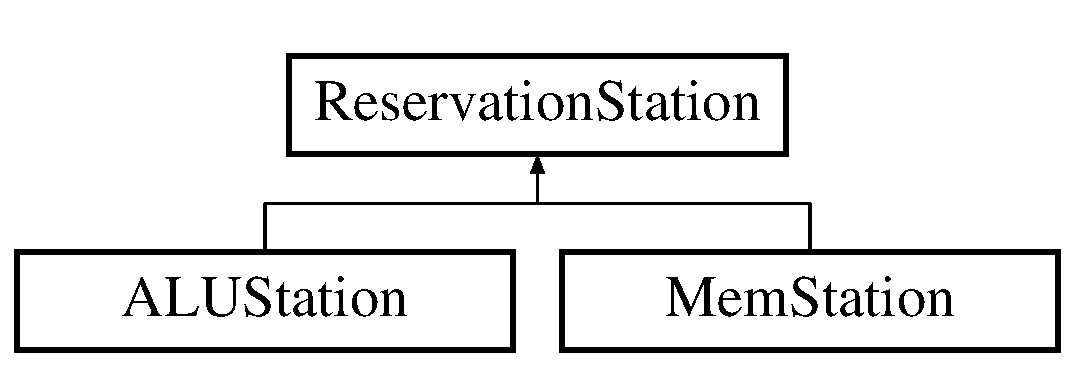
\includegraphics[height=2.000000cm]{classReservationStation}
\end{center}
\end{figure}
\subsection*{\-Public \-Member \-Functions}
\begin{DoxyCompactItemize}
\item 
\hyperlink{classReservationStation_ad155a9f0c4283cead97e512ce6d246ce}{\-Reservation\-Station} (\-String \hyperlink{classReservationStation_a2c0bd5b95f126395b0ab081394f090f6}{sname})
\item 
boolean \hyperlink{classReservationStation_aede190e7bfa282635f8a57ac3eaf74a5}{is\-Result\-Ready} ()
\item 
boolean \hyperlink{classReservationStation_a287759995344e119f4a108de7c648a76}{is\-Result\-Written} ()
\item 
boolean \hyperlink{classReservationStation_a26c60c26b4d03bbf7df5556d3b551621}{is\-Busy} ()
\item 
long \hyperlink{classReservationStation_a5775d6b5146a5392f8d6fdfa93b35309}{get\-Duration} ()
\item 
void \hyperlink{classReservationStation_ab9284f1b138b87ddcb50f4633d371a2f}{set\-Duration} (long d)
\item 
\-String \hyperlink{classReservationStation_a6b24d9296a10878d877a265a94ceec0b}{get\-Name} ()
\item 
void \hyperlink{classReservationStation_af1050ba62791a21550619fbe7ca76553}{set\-Name} (\-String name)
\item 
void \hyperlink{classReservationStation_a74dce4967c626f54888b1029169e8536}{perform\-Cycle} ()
\end{DoxyCompactItemize}
\subsection*{\-Protected \-Member \-Functions}
\begin{DoxyCompactItemize}
\item 
boolean \hyperlink{classReservationStation_a273bb4bbfdc3c1c481815ce690424bb7}{is\-Place\-Holder} (\-String to\-\_\-check)
\end{DoxyCompactItemize}
\subsection*{\-Protected \-Attributes}
\begin{DoxyCompactItemize}
\item 
\-String \hyperlink{classReservationStation_a2c0bd5b95f126395b0ab081394f090f6}{sname}
\begin{DoxyCompactList}\small\item\em name of reservation station \end{DoxyCompactList}\item 
boolean \hyperlink{classReservationStation_a0a2668bbae4e5d78dca63e3d38b4909f}{busy}
\begin{DoxyCompactList}\small\item\em flag indicating whether station holding an operation \end{DoxyCompactList}\item 
\hyperlink{classOperation}{\-Operation} \hyperlink{classReservationStation_a5dd33977e49327535ed47746caecd956}{operation}
\begin{DoxyCompactList}\small\item\em type of operation \end{DoxyCompactList}\item 
\-String \hyperlink{classReservationStation_a7d8ec53057e9762a0592c8052704fd88}{result}
\begin{DoxyCompactList}\small\item\em used to hold result \end{DoxyCompactList}\item 
long \hyperlink{classReservationStation_aa5e7a4c5ed6fd7e5e97782deb8feeeaa}{duration}
\begin{DoxyCompactList}\small\item\em holds the durations of the instruction \end{DoxyCompactList}\item 
boolean \hyperlink{classReservationStation_affeac0d7f9f9199919042bdb66ba2f73}{result\-Ready}
\begin{DoxyCompactList}\small\item\em flag indicating result is ready to be written \end{DoxyCompactList}\item 
boolean \hyperlink{classReservationStation_af3a98e6cc1d9b79263ed8848295fa29c}{result\-Written}
\begin{DoxyCompactList}\small\item\em flag indicating the result has been written \end{DoxyCompactList}\end{DoxyCompactItemize}
\subsection*{\-Package \-Functions}
\begin{DoxyCompactItemize}
\item 
abstract void \hyperlink{classReservationStation_a5788893e16b640dc7edbab832b1cb80d}{clear} ()
\item 
abstract boolean \hyperlink{classReservationStation_a4fe26aca967123d4e9ec5aabf55d4d17}{is\-Ready} ()
\item 
abstract void \hyperlink{classReservationStation_a5108e433a0a7e7cdd072fa7bcecdd399}{schedule\-Instruction} (\hyperlink{classOperation}{\-Operation} op, \hyperlink{classRegisterFiles}{\-Register\-Files} reg\-\_\-in, int cycles)
\item 
\-String \hyperlink{classReservationStation_a5319dce35333d97f4ba3880d47bd1f4d}{get\-Result} ()
\end{DoxyCompactItemize}


\subsection{\-Detailed \-Description}
\-This class provides all \-Reservation \-Station functionality. 

\subsection{\-Constructor \& \-Destructor \-Documentation}
\hypertarget{classReservationStation_ad155a9f0c4283cead97e512ce6d246ce}{\index{\-Reservation\-Station@{\-Reservation\-Station}!\-Reservation\-Station@{\-Reservation\-Station}}
\index{\-Reservation\-Station@{\-Reservation\-Station}!ReservationStation@{\-Reservation\-Station}}
\subsubsection[{\-Reservation\-Station}]{\setlength{\rightskip}{0pt plus 5cm}{\bf \-Reservation\-Station.\-Reservation\-Station} (
\begin{DoxyParamCaption}
\item[{\-String}]{sname}
\end{DoxyParamCaption}
)}}\label{classReservationStation_ad155a9f0c4283cead97e512ce6d246ce}
\-Construct an \-Reservationstation object and initialize sname,busy and operation 

\subsection{\-Member \-Function \-Documentation}
\hypertarget{classReservationStation_a5788893e16b640dc7edbab832b1cb80d}{\index{\-Reservation\-Station@{\-Reservation\-Station}!clear@{clear}}
\index{clear@{clear}!ReservationStation@{\-Reservation\-Station}}
\subsubsection[{clear}]{\setlength{\rightskip}{0pt plus 5cm}abstract void {\bf \-Reservation\-Station.\-clear} (
\begin{DoxyParamCaption}
{}
\end{DoxyParamCaption}
)\hspace{0.3cm}{\ttfamily  \mbox{[}package, pure virtual\mbox{]}}}}\label{classReservationStation_a5788893e16b640dc7edbab832b1cb80d}
\-Abstract function to clear the reservation station 

\-Implemented in \hyperlink{classMemStation_ab02b57a1bea7277dab474c8ffd7ac5ac}{\-Mem\-Station}, and \hyperlink{classALUStation_a2fa486045af0a1ceea0cc089f1d7c285}{\-A\-L\-U\-Station}.

\hypertarget{classReservationStation_a5775d6b5146a5392f8d6fdfa93b35309}{\index{\-Reservation\-Station@{\-Reservation\-Station}!get\-Duration@{get\-Duration}}
\index{get\-Duration@{get\-Duration}!ReservationStation@{\-Reservation\-Station}}
\subsubsection[{get\-Duration}]{\setlength{\rightskip}{0pt plus 5cm}long {\bf \-Reservation\-Station.\-get\-Duration} (
\begin{DoxyParamCaption}
{}
\end{DoxyParamCaption}
)}}\label{classReservationStation_a5775d6b5146a5392f8d6fdfa93b35309}
\-Function returns the value of duration \hypertarget{classReservationStation_a6b24d9296a10878d877a265a94ceec0b}{\index{\-Reservation\-Station@{\-Reservation\-Station}!get\-Name@{get\-Name}}
\index{get\-Name@{get\-Name}!ReservationStation@{\-Reservation\-Station}}
\subsubsection[{get\-Name}]{\setlength{\rightskip}{0pt plus 5cm}\-String {\bf \-Reservation\-Station.\-get\-Name} (
\begin{DoxyParamCaption}
{}
\end{DoxyParamCaption}
)}}\label{classReservationStation_a6b24d9296a10878d877a265a94ceec0b}
\-Function returns the value of name of reservation station \hypertarget{classReservationStation_a5319dce35333d97f4ba3880d47bd1f4d}{\index{\-Reservation\-Station@{\-Reservation\-Station}!get\-Result@{get\-Result}}
\index{get\-Result@{get\-Result}!ReservationStation@{\-Reservation\-Station}}
\subsubsection[{get\-Result}]{\setlength{\rightskip}{0pt plus 5cm}\-String {\bf \-Reservation\-Station.\-get\-Result} (
\begin{DoxyParamCaption}
{}
\end{DoxyParamCaption}
)\hspace{0.3cm}{\ttfamily  \mbox{[}package\mbox{]}}}}\label{classReservationStation_a5319dce35333d97f4ba3880d47bd1f4d}
\-Return the result \hypertarget{classReservationStation_a26c60c26b4d03bbf7df5556d3b551621}{\index{\-Reservation\-Station@{\-Reservation\-Station}!is\-Busy@{is\-Busy}}
\index{is\-Busy@{is\-Busy}!ReservationStation@{\-Reservation\-Station}}
\subsubsection[{is\-Busy}]{\setlength{\rightskip}{0pt plus 5cm}boolean {\bf \-Reservation\-Station.\-is\-Busy} (
\begin{DoxyParamCaption}
{}
\end{DoxyParamCaption}
)}}\label{classReservationStation_a26c60c26b4d03bbf7df5556d3b551621}
\-Function return the value of busy \hypertarget{classReservationStation_a273bb4bbfdc3c1c481815ce690424bb7}{\index{\-Reservation\-Station@{\-Reservation\-Station}!is\-Place\-Holder@{is\-Place\-Holder}}
\index{is\-Place\-Holder@{is\-Place\-Holder}!ReservationStation@{\-Reservation\-Station}}
\subsubsection[{is\-Place\-Holder}]{\setlength{\rightskip}{0pt plus 5cm}boolean {\bf \-Reservation\-Station.\-is\-Place\-Holder} (
\begin{DoxyParamCaption}
\item[{\-String}]{to\-\_\-check}
\end{DoxyParamCaption}
)\hspace{0.3cm}{\ttfamily  \mbox{[}protected\mbox{]}}}}\label{classReservationStation_a273bb4bbfdc3c1c481815ce690424bb7}
\-Utility function toc check if the \-Register \-Value is an alias \hypertarget{classReservationStation_a4fe26aca967123d4e9ec5aabf55d4d17}{\index{\-Reservation\-Station@{\-Reservation\-Station}!is\-Ready@{is\-Ready}}
\index{is\-Ready@{is\-Ready}!ReservationStation@{\-Reservation\-Station}}
\subsubsection[{is\-Ready}]{\setlength{\rightskip}{0pt plus 5cm}abstract boolean {\bf \-Reservation\-Station.\-is\-Ready} (
\begin{DoxyParamCaption}
{}
\end{DoxyParamCaption}
)\hspace{0.3cm}{\ttfamily  \mbox{[}package, pure virtual\mbox{]}}}}\label{classReservationStation_a4fe26aca967123d4e9ec5aabf55d4d17}
\-Abstract \-Function to determine whether the \-Station is \-Ready for use 

\-Implemented in \hyperlink{classMemStation_ac118dad2969d9bab0c2813b0e8681aa7}{\-Mem\-Station}, and \hyperlink{classALUStation_a5594f76ac16f7d0ee029759a8aa0e95b}{\-A\-L\-U\-Station}.

\hypertarget{classReservationStation_aede190e7bfa282635f8a57ac3eaf74a5}{\index{\-Reservation\-Station@{\-Reservation\-Station}!is\-Result\-Ready@{is\-Result\-Ready}}
\index{is\-Result\-Ready@{is\-Result\-Ready}!ReservationStation@{\-Reservation\-Station}}
\subsubsection[{is\-Result\-Ready}]{\setlength{\rightskip}{0pt plus 5cm}boolean {\bf \-Reservation\-Station.\-is\-Result\-Ready} (
\begin{DoxyParamCaption}
{}
\end{DoxyParamCaption}
)}}\label{classReservationStation_aede190e7bfa282635f8a57ac3eaf74a5}
\-Function return the value of resultready \hypertarget{classReservationStation_a287759995344e119f4a108de7c648a76}{\index{\-Reservation\-Station@{\-Reservation\-Station}!is\-Result\-Written@{is\-Result\-Written}}
\index{is\-Result\-Written@{is\-Result\-Written}!ReservationStation@{\-Reservation\-Station}}
\subsubsection[{is\-Result\-Written}]{\setlength{\rightskip}{0pt plus 5cm}boolean {\bf \-Reservation\-Station.\-is\-Result\-Written} (
\begin{DoxyParamCaption}
{}
\end{DoxyParamCaption}
)}}\label{classReservationStation_a287759995344e119f4a108de7c648a76}
\-Function returns the value of resultwritten \hypertarget{classReservationStation_a74dce4967c626f54888b1029169e8536}{\index{\-Reservation\-Station@{\-Reservation\-Station}!perform\-Cycle@{perform\-Cycle}}
\index{perform\-Cycle@{perform\-Cycle}!ReservationStation@{\-Reservation\-Station}}
\subsubsection[{perform\-Cycle}]{\setlength{\rightskip}{0pt plus 5cm}void {\bf \-Reservation\-Station.\-perform\-Cycle} (
\begin{DoxyParamCaption}
{}
\end{DoxyParamCaption}
)}}\label{classReservationStation_a74dce4967c626f54888b1029169e8536}
\-Decrement duration \hypertarget{classReservationStation_a5108e433a0a7e7cdd072fa7bcecdd399}{\index{\-Reservation\-Station@{\-Reservation\-Station}!schedule\-Instruction@{schedule\-Instruction}}
\index{schedule\-Instruction@{schedule\-Instruction}!ReservationStation@{\-Reservation\-Station}}
\subsubsection[{schedule\-Instruction}]{\setlength{\rightskip}{0pt plus 5cm}abstract void {\bf \-Reservation\-Station.\-schedule\-Instruction} (
\begin{DoxyParamCaption}
\item[{{\bf \-Operation}}]{op, }
\item[{{\bf \-Register\-Files}}]{reg\-\_\-in, }
\item[{int}]{cycles}
\end{DoxyParamCaption}
)\hspace{0.3cm}{\ttfamily  \mbox{[}package, pure virtual\mbox{]}}}}\label{classReservationStation_a5108e433a0a7e7cdd072fa7bcecdd399}
\-Abstract \-Function to schedule the instruction 

\-Implemented in \hyperlink{classMemStation_af5cbfa20af449839121307147b3af436}{\-Mem\-Station}, and \hyperlink{classALUStation_a7390a161d8b942caf223b17ea3c10eaf}{\-A\-L\-U\-Station}.

\hypertarget{classReservationStation_ab9284f1b138b87ddcb50f4633d371a2f}{\index{\-Reservation\-Station@{\-Reservation\-Station}!set\-Duration@{set\-Duration}}
\index{set\-Duration@{set\-Duration}!ReservationStation@{\-Reservation\-Station}}
\subsubsection[{set\-Duration}]{\setlength{\rightskip}{0pt plus 5cm}void {\bf \-Reservation\-Station.\-set\-Duration} (
\begin{DoxyParamCaption}
\item[{long}]{d}
\end{DoxyParamCaption}
)}}\label{classReservationStation_ab9284f1b138b87ddcb50f4633d371a2f}
\-Function sets the value of duration \hypertarget{classReservationStation_af1050ba62791a21550619fbe7ca76553}{\index{\-Reservation\-Station@{\-Reservation\-Station}!set\-Name@{set\-Name}}
\index{set\-Name@{set\-Name}!ReservationStation@{\-Reservation\-Station}}
\subsubsection[{set\-Name}]{\setlength{\rightskip}{0pt plus 5cm}void {\bf \-Reservation\-Station.\-set\-Name} (
\begin{DoxyParamCaption}
\item[{\-String}]{name}
\end{DoxyParamCaption}
)}}\label{classReservationStation_af1050ba62791a21550619fbe7ca76553}
\-Function sets the name of the reservation station 

\subsection{\-Member \-Data \-Documentation}
\hypertarget{classReservationStation_a0a2668bbae4e5d78dca63e3d38b4909f}{\index{\-Reservation\-Station@{\-Reservation\-Station}!busy@{busy}}
\index{busy@{busy}!ReservationStation@{\-Reservation\-Station}}
\subsubsection[{busy}]{\setlength{\rightskip}{0pt plus 5cm}boolean {\bf \-Reservation\-Station.\-busy}\hspace{0.3cm}{\ttfamily  \mbox{[}protected\mbox{]}}}}\label{classReservationStation_a0a2668bbae4e5d78dca63e3d38b4909f}


flag indicating whether station holding an operation 

\hypertarget{classReservationStation_aa5e7a4c5ed6fd7e5e97782deb8feeeaa}{\index{\-Reservation\-Station@{\-Reservation\-Station}!duration@{duration}}
\index{duration@{duration}!ReservationStation@{\-Reservation\-Station}}
\subsubsection[{duration}]{\setlength{\rightskip}{0pt plus 5cm}long {\bf \-Reservation\-Station.\-duration}\hspace{0.3cm}{\ttfamily  \mbox{[}protected\mbox{]}}}}\label{classReservationStation_aa5e7a4c5ed6fd7e5e97782deb8feeeaa}


holds the durations of the instruction 

\hypertarget{classReservationStation_a5dd33977e49327535ed47746caecd956}{\index{\-Reservation\-Station@{\-Reservation\-Station}!operation@{operation}}
\index{operation@{operation}!ReservationStation@{\-Reservation\-Station}}
\subsubsection[{operation}]{\setlength{\rightskip}{0pt plus 5cm}{\bf \-Operation} {\bf \-Reservation\-Station.\-operation}\hspace{0.3cm}{\ttfamily  \mbox{[}protected\mbox{]}}}}\label{classReservationStation_a5dd33977e49327535ed47746caecd956}


type of operation 

\hypertarget{classReservationStation_a7d8ec53057e9762a0592c8052704fd88}{\index{\-Reservation\-Station@{\-Reservation\-Station}!result@{result}}
\index{result@{result}!ReservationStation@{\-Reservation\-Station}}
\subsubsection[{result}]{\setlength{\rightskip}{0pt plus 5cm}\-String {\bf \-Reservation\-Station.\-result}\hspace{0.3cm}{\ttfamily  \mbox{[}protected\mbox{]}}}}\label{classReservationStation_a7d8ec53057e9762a0592c8052704fd88}


used to hold result 

\hypertarget{classReservationStation_affeac0d7f9f9199919042bdb66ba2f73}{\index{\-Reservation\-Station@{\-Reservation\-Station}!result\-Ready@{result\-Ready}}
\index{result\-Ready@{result\-Ready}!ReservationStation@{\-Reservation\-Station}}
\subsubsection[{result\-Ready}]{\setlength{\rightskip}{0pt plus 5cm}boolean {\bf \-Reservation\-Station.\-result\-Ready}\hspace{0.3cm}{\ttfamily  \mbox{[}protected\mbox{]}}}}\label{classReservationStation_affeac0d7f9f9199919042bdb66ba2f73}


flag indicating result is ready to be written 

\hypertarget{classReservationStation_af3a98e6cc1d9b79263ed8848295fa29c}{\index{\-Reservation\-Station@{\-Reservation\-Station}!result\-Written@{result\-Written}}
\index{result\-Written@{result\-Written}!ReservationStation@{\-Reservation\-Station}}
\subsubsection[{result\-Written}]{\setlength{\rightskip}{0pt plus 5cm}boolean {\bf \-Reservation\-Station.\-result\-Written}\hspace{0.3cm}{\ttfamily  \mbox{[}protected\mbox{]}}}}\label{classReservationStation_af3a98e6cc1d9b79263ed8848295fa29c}


flag indicating the result has been written 

\hypertarget{classReservationStation_a2c0bd5b95f126395b0ab081394f090f6}{\index{\-Reservation\-Station@{\-Reservation\-Station}!sname@{sname}}
\index{sname@{sname}!ReservationStation@{\-Reservation\-Station}}
\subsubsection[{sname}]{\setlength{\rightskip}{0pt plus 5cm}\-String {\bf \-Reservation\-Station.\-sname}\hspace{0.3cm}{\ttfamily  \mbox{[}protected\mbox{]}}}}\label{classReservationStation_a2c0bd5b95f126395b0ab081394f090f6}


name of reservation station 



\-The documentation for this class was generated from the following file\-:\begin{DoxyCompactItemize}
\item 
\hyperlink{ReservationStation_8java}{\-Reservation\-Station.\-java}\end{DoxyCompactItemize}

\hypertarget{classSimulation}{\section{\-Simulation \-Class \-Reference}
\label{classSimulation}\index{\-Simulation@{\-Simulation}}
}
\subsection*{\-Public \-Member \-Functions}
\begin{DoxyCompactItemize}
\item 
\hyperlink{classSimulation_aa24c4314fd1e140a1b9ad5feb06c6fb0}{\-Simulation} ()
\item 
void \hyperlink{classSimulation_a104eb3d562c22b1b10511adff57f4b4d}{initialize} (\-File data\-\_\-file)  throws Exception
\item 
boolean \hyperlink{classSimulation_ac47aeddaac1229f921bd8644aff688a9}{is\-Complete} ()
\item 
void \hyperlink{classSimulation_a6aa2ea799b5276681e8eb7c941c29d98}{perform\-Step} ()
\item 
int \hyperlink{classSimulation_a0cc18516e5b9e6f05b657d65adbb9f7b}{get\-Current\-Cycle} ()
\item 
\hyperlink{classOperationList}{\-Operation\-List} \hyperlink{classSimulation_a1cff8890330ebfd903d0e7bbef784a45}{get\-Operation\-List} ()
\item 
\hyperlink{classRegisterFiles}{\-Register\-Files} \hyperlink{classSimulation_affe7128840546c078763f7e21c3dac47}{get\-Register\-Files} ()
\item 
\hyperlink{classMemStation}{\-Mem\-Station}\mbox{[}$\,$\mbox{]} \hyperlink{classSimulation_a2f73acac6cc327ccd7721a797b8bdf6c}{get\-Mem\-Stations} ()
\item 
\hyperlink{classALUStation}{\-A\-L\-U\-Station}\mbox{[}$\,$\mbox{]} \hyperlink{classSimulation_a717866287d7c9ad508105400cd58a704}{get\-A\-L\-U\-Stations} ()
\end{DoxyCompactItemize}
\subsection*{\-Private \-Member \-Functions}
\begin{DoxyCompactItemize}
\item 
void \hyperlink{classSimulation_a24ef9f4425a72b53e78d79f2496f00a2}{parse\-Comment} (\-String comment)
\item 
boolean \hyperlink{classSimulation_a50ecd57c05305f3a27255b25d5c29188}{classify} (\-String opcode)
\item 
void \hyperlink{classSimulation_acb55c33781847629f2523d0aa58e6f71}{broadcast} (\-String alias, \-String result)
\end{DoxyCompactItemize}
\subsection*{\-Private \-Attributes}
\begin{DoxyCompactItemize}
\item 
\hyperlink{classOperationList}{\-Operation\-List} \hyperlink{classSimulation_a9569c59ef6447bb109d924ab08b952db}{operations}
\begin{DoxyCompactList}\small\item\em \-List of instructions. \end{DoxyCompactList}\item 
\hyperlink{classRegisterFiles}{\-Register\-Files} \hyperlink{classSimulation_a72082ebb1736f61f976fb4795c6446a6}{registers}
\begin{DoxyCompactList}\small\item\em \-Register \-Files. \end{DoxyCompactList}\item 
\hyperlink{classALUStation}{\-A\-L\-U\-Station}\mbox{[}$\,$\mbox{]} \hyperlink{classSimulation_a088d8379681674f73ff28d67fa15c4b1}{alu\-\_\-rs}
\begin{DoxyCompactList}\small\item\em \-A\-L\-U and \-Integer \-Reservation \-Stations. \end{DoxyCompactList}\item 
\hyperlink{classMemStation}{\-Mem\-Station}\mbox{[}$\,$\mbox{]} \hyperlink{classSimulation_a2d7653a8b926b1950e545b4ddf99525a}{mem\-\_\-rs}
\begin{DoxyCompactList}\small\item\em \-Memory \-Reservation \-Stations. \end{DoxyCompactList}\item 
\-Hash\-Map$<$ \-String, \-Integer\mbox{[}$\,$\mbox{]} $>$ \hyperlink{classSimulation_aa1da0fd99a66e4f3290cab75db0498ba}{instruction\-\_\-to\-\_\-station}
\begin{DoxyCompactList}\small\item\em \-Mapping of instructions to \-Reservation \-Stations. \end{DoxyCompactList}\item 
\-Hash\-Map$<$ \-String, \-Integer $>$ \hyperlink{classSimulation_aefb6ae75923bda2ea63a2789c6ea1387}{instruction\-\_\-to\-\_\-time}
\begin{DoxyCompactList}\small\item\em \-Mapping of instructions to \-Execution \-Time. \end{DoxyCompactList}\item 
\-Hash\-Map$<$ \-String, \-String $>$ \hyperlink{classSimulation_a4ba6804e72f9296ddbaf07334c656267}{alias\-\_\-to\-\_\-register}
\begin{DoxyCompactList}\small\item\em \-Mapping of placeholder to \-Register. \end{DoxyCompactList}\item 
\-Hash\-Map$<$ \-String, \-Integer $>$ \hyperlink{classSimulation_ad6a6dd370a3221f0b89718c9b64e3dad}{memory\-\_\-buffer}
\begin{DoxyCompactList}\small\item\em \-Mapping of operation issue numbers to ,emory locations. \end{DoxyCompactList}\item 
\hyperlink{classClock}{\-Clock} \hyperlink{classSimulation_af485d36c87120ad92b39bbea3e363cda}{clock}
\begin{DoxyCompactList}\small\item\em \hyperlink{classClock}{\-Clock} \-Cycle \-Object. \end{DoxyCompactList}\item 
boolean \hyperlink{classSimulation_a7c5a3018517be8966e7242ada10d5ba0}{is\-\_\-initialized}
\begin{DoxyCompactList}\small\item\em \-Whether the \hyperlink{classSimulation}{\-Simulation} \-Instance is initialized. \end{DoxyCompactList}\end{DoxyCompactItemize}


\subsection{\-Detailed \-Description}
\-This class contains all simulation logic. 

\subsection{\-Constructor \& \-Destructor \-Documentation}
\hypertarget{classSimulation_aa24c4314fd1e140a1b9ad5feb06c6fb0}{\index{\-Simulation@{\-Simulation}!\-Simulation@{\-Simulation}}
\index{\-Simulation@{\-Simulation}!Simulation@{\-Simulation}}
\subsubsection[{\-Simulation}]{\setlength{\rightskip}{0pt plus 5cm}{\bf \-Simulation.\-Simulation} (
\begin{DoxyParamCaption}
{}
\end{DoxyParamCaption}
)}}\label{classSimulation_aa24c4314fd1e140a1b9ad5feb06c6fb0}
\hyperlink{classSimulation}{\-Simulation} \-Constructor 

\subsection{\-Member \-Function \-Documentation}
\hypertarget{classSimulation_acb55c33781847629f2523d0aa58e6f71}{\index{\-Simulation@{\-Simulation}!broadcast@{broadcast}}
\index{broadcast@{broadcast}!Simulation@{\-Simulation}}
\subsubsection[{broadcast}]{\setlength{\rightskip}{0pt plus 5cm}void {\bf \-Simulation.\-broadcast} (
\begin{DoxyParamCaption}
\item[{\-String}]{alias, }
\item[{\-String}]{result}
\end{DoxyParamCaption}
)\hspace{0.3cm}{\ttfamily  \mbox{[}private\mbox{]}}}}\label{classSimulation_acb55c33781847629f2523d0aa58e6f71}
\-Broadcast the \-Result to all \-Reservation \-Stations \-Update the \-Register \-File \hypertarget{classSimulation_a50ecd57c05305f3a27255b25d5c29188}{\index{\-Simulation@{\-Simulation}!classify@{classify}}
\index{classify@{classify}!Simulation@{\-Simulation}}
\subsubsection[{classify}]{\setlength{\rightskip}{0pt plus 5cm}boolean {\bf \-Simulation.\-classify} (
\begin{DoxyParamCaption}
\item[{\-String}]{opcode}
\end{DoxyParamCaption}
)\hspace{0.3cm}{\ttfamily  \mbox{[}private\mbox{]}}}}\label{classSimulation_a50ecd57c05305f3a27255b25d5c29188}
\-Classify an \-Instruction as \-Memory or \-Other \hypertarget{classSimulation_a717866287d7c9ad508105400cd58a704}{\index{\-Simulation@{\-Simulation}!get\-A\-L\-U\-Stations@{get\-A\-L\-U\-Stations}}
\index{get\-A\-L\-U\-Stations@{get\-A\-L\-U\-Stations}!Simulation@{\-Simulation}}
\subsubsection[{get\-A\-L\-U\-Stations}]{\setlength{\rightskip}{0pt plus 5cm}{\bf \-A\-L\-U\-Station} \mbox{[}$\,$\mbox{]} {\bf \-Simulation.\-get\-A\-L\-U\-Stations} (
\begin{DoxyParamCaption}
{}
\end{DoxyParamCaption}
)}}\label{classSimulation_a717866287d7c9ad508105400cd58a704}
\-Return the \-A\-L\-U \-Reservation \-Stations \hypertarget{classSimulation_a0cc18516e5b9e6f05b657d65adbb9f7b}{\index{\-Simulation@{\-Simulation}!get\-Current\-Cycle@{get\-Current\-Cycle}}
\index{get\-Current\-Cycle@{get\-Current\-Cycle}!Simulation@{\-Simulation}}
\subsubsection[{get\-Current\-Cycle}]{\setlength{\rightskip}{0pt plus 5cm}int {\bf \-Simulation.\-get\-Current\-Cycle} (
\begin{DoxyParamCaption}
{}
\end{DoxyParamCaption}
)}}\label{classSimulation_a0cc18516e5b9e6f05b657d65adbb9f7b}
\-Return the current clock cycle \hypertarget{classSimulation_a2f73acac6cc327ccd7721a797b8bdf6c}{\index{\-Simulation@{\-Simulation}!get\-Mem\-Stations@{get\-Mem\-Stations}}
\index{get\-Mem\-Stations@{get\-Mem\-Stations}!Simulation@{\-Simulation}}
\subsubsection[{get\-Mem\-Stations}]{\setlength{\rightskip}{0pt plus 5cm}{\bf \-Mem\-Station} \mbox{[}$\,$\mbox{]} {\bf \-Simulation.\-get\-Mem\-Stations} (
\begin{DoxyParamCaption}
{}
\end{DoxyParamCaption}
)}}\label{classSimulation_a2f73acac6cc327ccd7721a797b8bdf6c}
\-Return the \-Memory \-Reservation \-Stations \hypertarget{classSimulation_a1cff8890330ebfd903d0e7bbef784a45}{\index{\-Simulation@{\-Simulation}!get\-Operation\-List@{get\-Operation\-List}}
\index{get\-Operation\-List@{get\-Operation\-List}!Simulation@{\-Simulation}}
\subsubsection[{get\-Operation\-List}]{\setlength{\rightskip}{0pt plus 5cm}{\bf \-Operation\-List} {\bf \-Simulation.\-get\-Operation\-List} (
\begin{DoxyParamCaption}
{}
\end{DoxyParamCaption}
)}}\label{classSimulation_a1cff8890330ebfd903d0e7bbef784a45}
\-Return the \-Instruction \-List \hypertarget{classSimulation_affe7128840546c078763f7e21c3dac47}{\index{\-Simulation@{\-Simulation}!get\-Register\-Files@{get\-Register\-Files}}
\index{get\-Register\-Files@{get\-Register\-Files}!Simulation@{\-Simulation}}
\subsubsection[{get\-Register\-Files}]{\setlength{\rightskip}{0pt plus 5cm}{\bf \-Register\-Files} {\bf \-Simulation.\-get\-Register\-Files} (
\begin{DoxyParamCaption}
{}
\end{DoxyParamCaption}
)}}\label{classSimulation_affe7128840546c078763f7e21c3dac47}
\-Return the \-Regieter \-Files \hypertarget{classSimulation_a104eb3d562c22b1b10511adff57f4b4d}{\index{\-Simulation@{\-Simulation}!initialize@{initialize}}
\index{initialize@{initialize}!Simulation@{\-Simulation}}
\subsubsection[{initialize}]{\setlength{\rightskip}{0pt plus 5cm}void {\bf \-Simulation.\-initialize} (
\begin{DoxyParamCaption}
\item[{\-File}]{data\-\_\-file}
\end{DoxyParamCaption}
)  throws \-Exception}}\label{classSimulation_a104eb3d562c22b1b10511adff57f4b4d}
\-Initialize the simulation \hypertarget{classSimulation_ac47aeddaac1229f921bd8644aff688a9}{\index{\-Simulation@{\-Simulation}!is\-Complete@{is\-Complete}}
\index{is\-Complete@{is\-Complete}!Simulation@{\-Simulation}}
\subsubsection[{is\-Complete}]{\setlength{\rightskip}{0pt plus 5cm}boolean {\bf \-Simulation.\-is\-Complete} (
\begin{DoxyParamCaption}
{}
\end{DoxyParamCaption}
)}}\label{classSimulation_ac47aeddaac1229f921bd8644aff688a9}
\-Returns true when the simulation has finished \hypertarget{classSimulation_a24ef9f4425a72b53e78d79f2496f00a2}{\index{\-Simulation@{\-Simulation}!parse\-Comment@{parse\-Comment}}
\index{parse\-Comment@{parse\-Comment}!Simulation@{\-Simulation}}
\subsubsection[{parse\-Comment}]{\setlength{\rightskip}{0pt plus 5cm}void {\bf \-Simulation.\-parse\-Comment} (
\begin{DoxyParamCaption}
\item[{\-String}]{comment}
\end{DoxyParamCaption}
)\hspace{0.3cm}{\ttfamily  \mbox{[}private\mbox{]}}}}\label{classSimulation_a24ef9f4425a72b53e78d79f2496f00a2}
\-Parse the comment and update the \-Register \-Files \-Accordingly \hypertarget{classSimulation_a6aa2ea799b5276681e8eb7c941c29d98}{\index{\-Simulation@{\-Simulation}!perform\-Step@{perform\-Step}}
\index{perform\-Step@{perform\-Step}!Simulation@{\-Simulation}}
\subsubsection[{perform\-Step}]{\setlength{\rightskip}{0pt plus 5cm}void {\bf \-Simulation.\-perform\-Step} (
\begin{DoxyParamCaption}
{}
\end{DoxyParamCaption}
)}}\label{classSimulation_a6aa2ea799b5276681e8eb7c941c29d98}
\-Perform one time step 

\subsection{\-Member \-Data \-Documentation}
\hypertarget{classSimulation_a4ba6804e72f9296ddbaf07334c656267}{\index{\-Simulation@{\-Simulation}!alias\-\_\-to\-\_\-register@{alias\-\_\-to\-\_\-register}}
\index{alias\-\_\-to\-\_\-register@{alias\-\_\-to\-\_\-register}!Simulation@{\-Simulation}}
\subsubsection[{alias\-\_\-to\-\_\-register}]{\setlength{\rightskip}{0pt plus 5cm}\-Hash\-Map$<$\-String, \-String$>$ {\bf \-Simulation.\-alias\-\_\-to\-\_\-register}\hspace{0.3cm}{\ttfamily  \mbox{[}private\mbox{]}}}}\label{classSimulation_a4ba6804e72f9296ddbaf07334c656267}


\-Mapping of placeholder to \-Register. 

\hypertarget{classSimulation_a088d8379681674f73ff28d67fa15c4b1}{\index{\-Simulation@{\-Simulation}!alu\-\_\-rs@{alu\-\_\-rs}}
\index{alu\-\_\-rs@{alu\-\_\-rs}!Simulation@{\-Simulation}}
\subsubsection[{alu\-\_\-rs}]{\setlength{\rightskip}{0pt plus 5cm}{\bf \-A\-L\-U\-Station} \mbox{[}$\,$\mbox{]} {\bf \-Simulation.\-alu\-\_\-rs}\hspace{0.3cm}{\ttfamily  \mbox{[}private\mbox{]}}}}\label{classSimulation_a088d8379681674f73ff28d67fa15c4b1}


\-A\-L\-U and \-Integer \-Reservation \-Stations. 

\hypertarget{classSimulation_af485d36c87120ad92b39bbea3e363cda}{\index{\-Simulation@{\-Simulation}!clock@{clock}}
\index{clock@{clock}!Simulation@{\-Simulation}}
\subsubsection[{clock}]{\setlength{\rightskip}{0pt plus 5cm}{\bf \-Clock} {\bf \-Simulation.\-clock}\hspace{0.3cm}{\ttfamily  \mbox{[}private\mbox{]}}}}\label{classSimulation_af485d36c87120ad92b39bbea3e363cda}


\hyperlink{classClock}{\-Clock} \-Cycle \-Object. 

\hypertarget{classSimulation_aa1da0fd99a66e4f3290cab75db0498ba}{\index{\-Simulation@{\-Simulation}!instruction\-\_\-to\-\_\-station@{instruction\-\_\-to\-\_\-station}}
\index{instruction\-\_\-to\-\_\-station@{instruction\-\_\-to\-\_\-station}!Simulation@{\-Simulation}}
\subsubsection[{instruction\-\_\-to\-\_\-station}]{\setlength{\rightskip}{0pt plus 5cm}\-Hash\-Map$<$\-String, \-Integer\mbox{[}$\,$\mbox{]} $>$ {\bf \-Simulation.\-instruction\-\_\-to\-\_\-station}\hspace{0.3cm}{\ttfamily  \mbox{[}private\mbox{]}}}}\label{classSimulation_aa1da0fd99a66e4f3290cab75db0498ba}


\-Mapping of instructions to \-Reservation \-Stations. 

\hypertarget{classSimulation_aefb6ae75923bda2ea63a2789c6ea1387}{\index{\-Simulation@{\-Simulation}!instruction\-\_\-to\-\_\-time@{instruction\-\_\-to\-\_\-time}}
\index{instruction\-\_\-to\-\_\-time@{instruction\-\_\-to\-\_\-time}!Simulation@{\-Simulation}}
\subsubsection[{instruction\-\_\-to\-\_\-time}]{\setlength{\rightskip}{0pt plus 5cm}\-Hash\-Map$<$\-String, \-Integer $>$ {\bf \-Simulation.\-instruction\-\_\-to\-\_\-time}\hspace{0.3cm}{\ttfamily  \mbox{[}private\mbox{]}}}}\label{classSimulation_aefb6ae75923bda2ea63a2789c6ea1387}


\-Mapping of instructions to \-Execution \-Time. 

\hypertarget{classSimulation_a7c5a3018517be8966e7242ada10d5ba0}{\index{\-Simulation@{\-Simulation}!is\-\_\-initialized@{is\-\_\-initialized}}
\index{is\-\_\-initialized@{is\-\_\-initialized}!Simulation@{\-Simulation}}
\subsubsection[{is\-\_\-initialized}]{\setlength{\rightskip}{0pt plus 5cm}boolean {\bf \-Simulation.\-is\-\_\-initialized}\hspace{0.3cm}{\ttfamily  \mbox{[}private\mbox{]}}}}\label{classSimulation_a7c5a3018517be8966e7242ada10d5ba0}


\-Whether the \hyperlink{classSimulation}{\-Simulation} \-Instance is initialized. 

\hypertarget{classSimulation_a2d7653a8b926b1950e545b4ddf99525a}{\index{\-Simulation@{\-Simulation}!mem\-\_\-rs@{mem\-\_\-rs}}
\index{mem\-\_\-rs@{mem\-\_\-rs}!Simulation@{\-Simulation}}
\subsubsection[{mem\-\_\-rs}]{\setlength{\rightskip}{0pt plus 5cm}{\bf \-Mem\-Station} \mbox{[}$\,$\mbox{]} {\bf \-Simulation.\-mem\-\_\-rs}\hspace{0.3cm}{\ttfamily  \mbox{[}private\mbox{]}}}}\label{classSimulation_a2d7653a8b926b1950e545b4ddf99525a}


\-Memory \-Reservation \-Stations. 

\hypertarget{classSimulation_ad6a6dd370a3221f0b89718c9b64e3dad}{\index{\-Simulation@{\-Simulation}!memory\-\_\-buffer@{memory\-\_\-buffer}}
\index{memory\-\_\-buffer@{memory\-\_\-buffer}!Simulation@{\-Simulation}}
\subsubsection[{memory\-\_\-buffer}]{\setlength{\rightskip}{0pt plus 5cm}\-Hash\-Map$<$\-String, \-Integer$>$ {\bf \-Simulation.\-memory\-\_\-buffer}\hspace{0.3cm}{\ttfamily  \mbox{[}private\mbox{]}}}}\label{classSimulation_ad6a6dd370a3221f0b89718c9b64e3dad}


\-Mapping of operation issue numbers to ,emory locations. 

\hypertarget{classSimulation_a9569c59ef6447bb109d924ab08b952db}{\index{\-Simulation@{\-Simulation}!operations@{operations}}
\index{operations@{operations}!Simulation@{\-Simulation}}
\subsubsection[{operations}]{\setlength{\rightskip}{0pt plus 5cm}{\bf \-Operation\-List} {\bf \-Simulation.\-operations}\hspace{0.3cm}{\ttfamily  \mbox{[}private\mbox{]}}}}\label{classSimulation_a9569c59ef6447bb109d924ab08b952db}


\-List of instructions. 

\hypertarget{classSimulation_a72082ebb1736f61f976fb4795c6446a6}{\index{\-Simulation@{\-Simulation}!registers@{registers}}
\index{registers@{registers}!Simulation@{\-Simulation}}
\subsubsection[{registers}]{\setlength{\rightskip}{0pt plus 5cm}{\bf \-Register\-Files} {\bf \-Simulation.\-registers}\hspace{0.3cm}{\ttfamily  \mbox{[}private\mbox{]}}}}\label{classSimulation_a72082ebb1736f61f976fb4795c6446a6}


\-Register \-Files. 



\-The documentation for this class was generated from the following file\-:\begin{DoxyCompactItemize}
\item 
\hyperlink{Simulation_8java}{\-Simulation.\-java}\end{DoxyCompactItemize}

\hypertarget{classTestModules}{\section{\-Test\-Modules \-Class \-Reference}
\label{classTestModules}\index{\-Test\-Modules@{\-Test\-Modules}}
}
\subsection*{\-Static \-Public \-Member \-Functions}
\begin{DoxyCompactItemize}
\item 
static void \hyperlink{classTestModules_a1dfd6f4708c66f2bfb057a98233b52b7}{main} (\-String args\mbox{[}$\,$\mbox{]})
\end{DoxyCompactItemize}


\subsection{\-Detailed \-Description}
\-This class contaisn all moduling testing. 

\subsection{\-Member \-Function \-Documentation}
\hypertarget{classTestModules_a1dfd6f4708c66f2bfb057a98233b52b7}{\index{\-Test\-Modules@{\-Test\-Modules}!main@{main}}
\index{main@{main}!TestModules@{\-Test\-Modules}}
\subsubsection[{main}]{\setlength{\rightskip}{0pt plus 5cm}static void {\bf \-Test\-Modules.\-main} (
\begin{DoxyParamCaption}
\item[{\-String}]{args\mbox{[}$\,$\mbox{]}}
\end{DoxyParamCaption}
)\hspace{0.3cm}{\ttfamily  \mbox{[}static\mbox{]}}}}\label{classTestModules_a1dfd6f4708c66f2bfb057a98233b52b7}


\-The documentation for this class was generated from the following file\-:\begin{DoxyCompactItemize}
\item 
\hyperlink{TestModules_8java}{\-Test\-Modules.\-java}\end{DoxyCompactItemize}

\hypertarget{classTomasuloGUI}{\section{\-Tomasulo\-G\-U\-I \-Class \-Reference}
\label{classTomasuloGUI}\index{\-Tomasulo\-G\-U\-I@{\-Tomasulo\-G\-U\-I}}
}
\subsection*{\-Public \-Member \-Functions}
\begin{DoxyCompactItemize}
\item 
\hyperlink{classTomasuloGUI_ae08510dffd34fb9fa786eff57481f1b9}{\-Tomasulo\-G\-U\-I} ()
\end{DoxyCompactItemize}
\subsection*{\-Static \-Public \-Member \-Functions}
\begin{DoxyCompactItemize}
\item 
static void \hyperlink{classTomasuloGUI_a28606c7d567bd1e006e010515cbbe873}{main} (\-String args\mbox{[}$\,$\mbox{]})
\end{DoxyCompactItemize}
\subsection*{\-Package \-Attributes}
\begin{DoxyCompactItemize}
\item 
\-J\-Panel \hyperlink{classTomasuloGUI_a04c211874e22ab75cd47d35dca120c9d}{control\-\_\-panel}
\begin{DoxyCompactList}\small\item\em \-Container panel for controls. \end{DoxyCompactList}\item 
\-J\-Panel \hyperlink{classTomasuloGUI_a34dc546fcc88949fbdaa5b588b5e18ea}{status\-\_\-panel}
\begin{DoxyCompactList}\small\item\em \-Container panel for status. \end{DoxyCompactList}\item 
\-J\-Label \hyperlink{classTomasuloGUI_aac9070de64d1efb4a849cb0eb20015c4}{file\-\_\-label}
\begin{DoxyCompactList}\small\item\em \-Filename label. \end{DoxyCompactList}\item 
\-J\-Table \hyperlink{classTomasuloGUI_a99dac43adb85dce62618469b155021f8}{op\-\_\-table}
\begin{DoxyCompactList}\small\item\em \-Instructions \-Table. \end{DoxyCompactList}\item 
\-J\-Table \hyperlink{classTomasuloGUI_a6ecd99ff02c80d24ecb2aa0ba2635fef}{rs\-\_\-table}
\begin{DoxyCompactList}\small\item\em \-A\-L\-U \-Reservation \-Station \-Table. \end{DoxyCompactList}\item 
\-J\-Table \hyperlink{classTomasuloGUI_a18580aaadebeefbfc8a2a6a6896d5a10}{mrs\-\_\-table}
\begin{DoxyCompactList}\small\item\em \-Memory \-Reservations \-Station \-Table. \end{DoxyCompactList}\item 
\-J\-Table \hyperlink{classTomasuloGUI_a0ef75f51c2dc43b3fc667bb1289d6cc0}{irs\-\_\-table}
\begin{DoxyCompactList}\small\item\em \-Integer \-Reservation \-Station \-Table. \end{DoxyCompactList}\item 
\-J\-Table \hyperlink{classTomasuloGUI_a5d9e4b23a54f429c9f0135e492bc7609}{reg\-\_\-table}
\begin{DoxyCompactList}\small\item\em \-Register \-File \-Table. \end{DoxyCompactList}\item 
\-Default\-Table\-Model \hyperlink{classTomasuloGUI_a6b5d956697d14589539bb8f765c8da5c}{op\-\_\-model}
\begin{DoxyCompactList}\small\item\em \-Instructions \-Table \-Model. \end{DoxyCompactList}\item 
\-Default\-Table\-Model \hyperlink{classTomasuloGUI_a1f5a9be366c1157ec2a5eb54de8c1b5b}{rs\-\_\-model}
\begin{DoxyCompactList}\small\item\em \-A\-L\-U \-Reservation \-Station \-Table \-Model. \end{DoxyCompactList}\item 
\-Default\-Table\-Model \hyperlink{classTomasuloGUI_ad017a1554cee627c47c5cea70fc58908}{mrs\-\_\-model}
\begin{DoxyCompactList}\small\item\em \-Memory \-Reservations \-Station \-Table \-Mdoel. \end{DoxyCompactList}\item 
\-Default\-Table\-Model \hyperlink{classTomasuloGUI_a2dc4ffde9e3f919d756d89fbfd5aac46}{irs\-\_\-model}
\begin{DoxyCompactList}\small\item\em \-Integer \-Reservation \-Station \-Table \-Model. \end{DoxyCompactList}\item 
\-Default\-Table\-Model \hyperlink{classTomasuloGUI_a70e2e15d3c1154ecc5a049f373d1178d}{reg\-\_\-model}
\begin{DoxyCompactList}\small\item\em \-Register \-File \-Table \-Model. \end{DoxyCompactList}\item 
\-J\-Button \hyperlink{classTomasuloGUI_ad94e3aa704e880a905631076935771a5}{load\-\_\-button}
\begin{DoxyCompactList}\small\item\em \-Load button. \end{DoxyCompactList}\item 
\-J\-Button \hyperlink{classTomasuloGUI_ac489de22d16f3c43bae896eb5c8980a3}{step\-\_\-button}
\begin{DoxyCompactList}\small\item\em \-Step button. \end{DoxyCompactList}\item 
\-J\-Text\-Field \hyperlink{classTomasuloGUI_a4e028c3179fd14d926d7a1896f844a20}{file\-\_\-field}
\item 
\-J\-Text\-Field \hyperlink{classTomasuloGUI_a518c1f6d1f2fcbc3df0c7fc4cdce7e25}{clocks\-\_\-field}
\begin{DoxyCompactList}\small\item\em \hyperlink{classClock}{\-Clock} display field. \end{DoxyCompactList}\item 
\hyperlink{classSimulation}{\-Simulation} \hyperlink{classTomasuloGUI_a9276faa3fed5236e393b96d517e2e6fc}{sim\-\_\-instance}
\begin{DoxyCompactList}\small\item\em \hyperlink{classSimulation}{\-Simulation} \-Wrapper \-Object. \end{DoxyCompactList}\item 
final \-J\-File\-Chooser \hyperlink{classTomasuloGUI_af5a309a292415fb6deb61903765d8679}{file\-\_\-dialog} = new \-J\-File\-Chooser()
\begin{DoxyCompactList}\small\item\em \-File selection dialog. \end{DoxyCompactList}\item 
\-File \hyperlink{classTomasuloGUI_a84fcf1ebe8e65d62c3c7f90382380946}{instructions\-\_\-file}
\begin{DoxyCompactList}\small\item\em \-Instructions \-File object. \end{DoxyCompactList}\end{DoxyCompactItemize}
\subsection*{\-Private \-Member \-Functions}
\begin{DoxyCompactItemize}
\item 
void \hyperlink{classTomasuloGUI_a65dd25b7e14e954baf4c4a6dfc96a192}{update\-Instruction\-Table} ()
\item 
void \hyperlink{classTomasuloGUI_a69f0c12dd9aef1f080a023b5abe5649e}{update\-Register\-Table} ()
\item 
void \hyperlink{classTomasuloGUI_a1c15ab07a1fde2b9ca5d189fe6d03ffe}{update\-Mem\-Table} ()
\item 
void \hyperlink{classTomasuloGUI_a34218d232187e85c142c686ba01798f6}{update\-A\-L\-U\-Table} ()
\end{DoxyCompactItemize}


\subsection{\-Detailed \-Description}
\-This class provides all \-G\-U\-I functionality. 

\subsection{\-Constructor \& \-Destructor \-Documentation}
\hypertarget{classTomasuloGUI_ae08510dffd34fb9fa786eff57481f1b9}{\index{\-Tomasulo\-G\-U\-I@{\-Tomasulo\-G\-U\-I}!\-Tomasulo\-G\-U\-I@{\-Tomasulo\-G\-U\-I}}
\index{\-Tomasulo\-G\-U\-I@{\-Tomasulo\-G\-U\-I}!TomasuloGUI@{\-Tomasulo\-G\-U\-I}}
\subsubsection[{\-Tomasulo\-G\-U\-I}]{\setlength{\rightskip}{0pt plus 5cm}{\bf \-Tomasulo\-G\-U\-I.\-Tomasulo\-G\-U\-I} (
\begin{DoxyParamCaption}
{}
\end{DoxyParamCaption}
)}}\label{classTomasuloGUI_ae08510dffd34fb9fa786eff57481f1b9}
\-The \-G\-U\-I \-Constructor 

\subsection{\-Member \-Function \-Documentation}
\hypertarget{classTomasuloGUI_a28606c7d567bd1e006e010515cbbe873}{\index{\-Tomasulo\-G\-U\-I@{\-Tomasulo\-G\-U\-I}!main@{main}}
\index{main@{main}!TomasuloGUI@{\-Tomasulo\-G\-U\-I}}
\subsubsection[{main}]{\setlength{\rightskip}{0pt plus 5cm}static void {\bf \-Tomasulo\-G\-U\-I.\-main} (
\begin{DoxyParamCaption}
\item[{\-String}]{args\mbox{[}$\,$\mbox{]}}
\end{DoxyParamCaption}
)\hspace{0.3cm}{\ttfamily  \mbox{[}static\mbox{]}}}}\label{classTomasuloGUI_a28606c7d567bd1e006e010515cbbe873}
\-The main function \hypertarget{classTomasuloGUI_a34218d232187e85c142c686ba01798f6}{\index{\-Tomasulo\-G\-U\-I@{\-Tomasulo\-G\-U\-I}!update\-A\-L\-U\-Table@{update\-A\-L\-U\-Table}}
\index{update\-A\-L\-U\-Table@{update\-A\-L\-U\-Table}!TomasuloGUI@{\-Tomasulo\-G\-U\-I}}
\subsubsection[{update\-A\-L\-U\-Table}]{\setlength{\rightskip}{0pt plus 5cm}void {\bf \-Tomasulo\-G\-U\-I.\-update\-A\-L\-U\-Table} (
\begin{DoxyParamCaption}
{}
\end{DoxyParamCaption}
)\hspace{0.3cm}{\ttfamily  \mbox{[}private\mbox{]}}}}\label{classTomasuloGUI_a34218d232187e85c142c686ba01798f6}
\-A\-L\-U\-Stations \-Table \-Update \-Helper \hypertarget{classTomasuloGUI_a65dd25b7e14e954baf4c4a6dfc96a192}{\index{\-Tomasulo\-G\-U\-I@{\-Tomasulo\-G\-U\-I}!update\-Instruction\-Table@{update\-Instruction\-Table}}
\index{update\-Instruction\-Table@{update\-Instruction\-Table}!TomasuloGUI@{\-Tomasulo\-G\-U\-I}}
\subsubsection[{update\-Instruction\-Table}]{\setlength{\rightskip}{0pt plus 5cm}void {\bf \-Tomasulo\-G\-U\-I.\-update\-Instruction\-Table} (
\begin{DoxyParamCaption}
{}
\end{DoxyParamCaption}
)\hspace{0.3cm}{\ttfamily  \mbox{[}private\mbox{]}}}}\label{classTomasuloGUI_a65dd25b7e14e954baf4c4a6dfc96a192}
\-Instruction \-Table \-Update \-Helper \hypertarget{classTomasuloGUI_a1c15ab07a1fde2b9ca5d189fe6d03ffe}{\index{\-Tomasulo\-G\-U\-I@{\-Tomasulo\-G\-U\-I}!update\-Mem\-Table@{update\-Mem\-Table}}
\index{update\-Mem\-Table@{update\-Mem\-Table}!TomasuloGUI@{\-Tomasulo\-G\-U\-I}}
\subsubsection[{update\-Mem\-Table}]{\setlength{\rightskip}{0pt plus 5cm}void {\bf \-Tomasulo\-G\-U\-I.\-update\-Mem\-Table} (
\begin{DoxyParamCaption}
{}
\end{DoxyParamCaption}
)\hspace{0.3cm}{\ttfamily  \mbox{[}private\mbox{]}}}}\label{classTomasuloGUI_a1c15ab07a1fde2b9ca5d189fe6d03ffe}
\-Mem\-Stations \-Table \-Update \-Helper \hypertarget{classTomasuloGUI_a69f0c12dd9aef1f080a023b5abe5649e}{\index{\-Tomasulo\-G\-U\-I@{\-Tomasulo\-G\-U\-I}!update\-Register\-Table@{update\-Register\-Table}}
\index{update\-Register\-Table@{update\-Register\-Table}!TomasuloGUI@{\-Tomasulo\-G\-U\-I}}
\subsubsection[{update\-Register\-Table}]{\setlength{\rightskip}{0pt plus 5cm}void {\bf \-Tomasulo\-G\-U\-I.\-update\-Register\-Table} (
\begin{DoxyParamCaption}
{}
\end{DoxyParamCaption}
)\hspace{0.3cm}{\ttfamily  \mbox{[}private\mbox{]}}}}\label{classTomasuloGUI_a69f0c12dd9aef1f080a023b5abe5649e}
\-Register \-Table \-Update \-Helper 

\subsection{\-Member \-Data \-Documentation}
\hypertarget{classTomasuloGUI_a518c1f6d1f2fcbc3df0c7fc4cdce7e25}{\index{\-Tomasulo\-G\-U\-I@{\-Tomasulo\-G\-U\-I}!clocks\-\_\-field@{clocks\-\_\-field}}
\index{clocks\-\_\-field@{clocks\-\_\-field}!TomasuloGUI@{\-Tomasulo\-G\-U\-I}}
\subsubsection[{clocks\-\_\-field}]{\setlength{\rightskip}{0pt plus 5cm}\-J\-Text\-Field {\bf \-Tomasulo\-G\-U\-I.\-clocks\-\_\-field}\hspace{0.3cm}{\ttfamily  \mbox{[}package\mbox{]}}}}\label{classTomasuloGUI_a518c1f6d1f2fcbc3df0c7fc4cdce7e25}


\hyperlink{classClock}{\-Clock} display field. 

\hypertarget{classTomasuloGUI_a04c211874e22ab75cd47d35dca120c9d}{\index{\-Tomasulo\-G\-U\-I@{\-Tomasulo\-G\-U\-I}!control\-\_\-panel@{control\-\_\-panel}}
\index{control\-\_\-panel@{control\-\_\-panel}!TomasuloGUI@{\-Tomasulo\-G\-U\-I}}
\subsubsection[{control\-\_\-panel}]{\setlength{\rightskip}{0pt plus 5cm}\-J\-Panel {\bf \-Tomasulo\-G\-U\-I.\-control\-\_\-panel}\hspace{0.3cm}{\ttfamily  \mbox{[}package\mbox{]}}}}\label{classTomasuloGUI_a04c211874e22ab75cd47d35dca120c9d}


\-Container panel for controls. 

\hypertarget{classTomasuloGUI_af5a309a292415fb6deb61903765d8679}{\index{\-Tomasulo\-G\-U\-I@{\-Tomasulo\-G\-U\-I}!file\-\_\-dialog@{file\-\_\-dialog}}
\index{file\-\_\-dialog@{file\-\_\-dialog}!TomasuloGUI@{\-Tomasulo\-G\-U\-I}}
\subsubsection[{file\-\_\-dialog}]{\setlength{\rightskip}{0pt plus 5cm}final \-J\-File\-Chooser {\bf \-Tomasulo\-G\-U\-I.\-file\-\_\-dialog} = new \-J\-File\-Chooser()\hspace{0.3cm}{\ttfamily  \mbox{[}package\mbox{]}}}}\label{classTomasuloGUI_af5a309a292415fb6deb61903765d8679}


\-File selection dialog. 

\hypertarget{classTomasuloGUI_a4e028c3179fd14d926d7a1896f844a20}{\index{\-Tomasulo\-G\-U\-I@{\-Tomasulo\-G\-U\-I}!file\-\_\-field@{file\-\_\-field}}
\index{file\-\_\-field@{file\-\_\-field}!TomasuloGUI@{\-Tomasulo\-G\-U\-I}}
\subsubsection[{file\-\_\-field}]{\setlength{\rightskip}{0pt plus 5cm}\-J\-Text\-Field {\bf \-Tomasulo\-G\-U\-I.\-file\-\_\-field}\hspace{0.3cm}{\ttfamily  \mbox{[}package\mbox{]}}}}\label{classTomasuloGUI_a4e028c3179fd14d926d7a1896f844a20}
\hypertarget{classTomasuloGUI_aac9070de64d1efb4a849cb0eb20015c4}{\index{\-Tomasulo\-G\-U\-I@{\-Tomasulo\-G\-U\-I}!file\-\_\-label@{file\-\_\-label}}
\index{file\-\_\-label@{file\-\_\-label}!TomasuloGUI@{\-Tomasulo\-G\-U\-I}}
\subsubsection[{file\-\_\-label}]{\setlength{\rightskip}{0pt plus 5cm}\-J\-Label {\bf \-Tomasulo\-G\-U\-I.\-file\-\_\-label}\hspace{0.3cm}{\ttfamily  \mbox{[}package\mbox{]}}}}\label{classTomasuloGUI_aac9070de64d1efb4a849cb0eb20015c4}


\-Filename label. 

\hypertarget{classTomasuloGUI_a84fcf1ebe8e65d62c3c7f90382380946}{\index{\-Tomasulo\-G\-U\-I@{\-Tomasulo\-G\-U\-I}!instructions\-\_\-file@{instructions\-\_\-file}}
\index{instructions\-\_\-file@{instructions\-\_\-file}!TomasuloGUI@{\-Tomasulo\-G\-U\-I}}
\subsubsection[{instructions\-\_\-file}]{\setlength{\rightskip}{0pt plus 5cm}\-File {\bf \-Tomasulo\-G\-U\-I.\-instructions\-\_\-file}\hspace{0.3cm}{\ttfamily  \mbox{[}package\mbox{]}}}}\label{classTomasuloGUI_a84fcf1ebe8e65d62c3c7f90382380946}


\-Instructions \-File object. 

\hypertarget{classTomasuloGUI_a2dc4ffde9e3f919d756d89fbfd5aac46}{\index{\-Tomasulo\-G\-U\-I@{\-Tomasulo\-G\-U\-I}!irs\-\_\-model@{irs\-\_\-model}}
\index{irs\-\_\-model@{irs\-\_\-model}!TomasuloGUI@{\-Tomasulo\-G\-U\-I}}
\subsubsection[{irs\-\_\-model}]{\setlength{\rightskip}{0pt plus 5cm}\-Default\-Table\-Model {\bf \-Tomasulo\-G\-U\-I.\-irs\-\_\-model}\hspace{0.3cm}{\ttfamily  \mbox{[}package\mbox{]}}}}\label{classTomasuloGUI_a2dc4ffde9e3f919d756d89fbfd5aac46}


\-Integer \-Reservation \-Station \-Table \-Model. 

\hypertarget{classTomasuloGUI_a0ef75f51c2dc43b3fc667bb1289d6cc0}{\index{\-Tomasulo\-G\-U\-I@{\-Tomasulo\-G\-U\-I}!irs\-\_\-table@{irs\-\_\-table}}
\index{irs\-\_\-table@{irs\-\_\-table}!TomasuloGUI@{\-Tomasulo\-G\-U\-I}}
\subsubsection[{irs\-\_\-table}]{\setlength{\rightskip}{0pt plus 5cm}\-J\-Table {\bf \-Tomasulo\-G\-U\-I.\-irs\-\_\-table}\hspace{0.3cm}{\ttfamily  \mbox{[}package\mbox{]}}}}\label{classTomasuloGUI_a0ef75f51c2dc43b3fc667bb1289d6cc0}


\-Integer \-Reservation \-Station \-Table. 

\hypertarget{classTomasuloGUI_ad94e3aa704e880a905631076935771a5}{\index{\-Tomasulo\-G\-U\-I@{\-Tomasulo\-G\-U\-I}!load\-\_\-button@{load\-\_\-button}}
\index{load\-\_\-button@{load\-\_\-button}!TomasuloGUI@{\-Tomasulo\-G\-U\-I}}
\subsubsection[{load\-\_\-button}]{\setlength{\rightskip}{0pt plus 5cm}\-J\-Button {\bf \-Tomasulo\-G\-U\-I.\-load\-\_\-button}\hspace{0.3cm}{\ttfamily  \mbox{[}package\mbox{]}}}}\label{classTomasuloGUI_ad94e3aa704e880a905631076935771a5}


\-Load button. 

\hypertarget{classTomasuloGUI_ad017a1554cee627c47c5cea70fc58908}{\index{\-Tomasulo\-G\-U\-I@{\-Tomasulo\-G\-U\-I}!mrs\-\_\-model@{mrs\-\_\-model}}
\index{mrs\-\_\-model@{mrs\-\_\-model}!TomasuloGUI@{\-Tomasulo\-G\-U\-I}}
\subsubsection[{mrs\-\_\-model}]{\setlength{\rightskip}{0pt plus 5cm}\-Default\-Table\-Model {\bf \-Tomasulo\-G\-U\-I.\-mrs\-\_\-model}\hspace{0.3cm}{\ttfamily  \mbox{[}package\mbox{]}}}}\label{classTomasuloGUI_ad017a1554cee627c47c5cea70fc58908}


\-Memory \-Reservations \-Station \-Table \-Mdoel. 

\hypertarget{classTomasuloGUI_a18580aaadebeefbfc8a2a6a6896d5a10}{\index{\-Tomasulo\-G\-U\-I@{\-Tomasulo\-G\-U\-I}!mrs\-\_\-table@{mrs\-\_\-table}}
\index{mrs\-\_\-table@{mrs\-\_\-table}!TomasuloGUI@{\-Tomasulo\-G\-U\-I}}
\subsubsection[{mrs\-\_\-table}]{\setlength{\rightskip}{0pt plus 5cm}\-J\-Table {\bf \-Tomasulo\-G\-U\-I.\-mrs\-\_\-table}\hspace{0.3cm}{\ttfamily  \mbox{[}package\mbox{]}}}}\label{classTomasuloGUI_a18580aaadebeefbfc8a2a6a6896d5a10}


\-Memory \-Reservations \-Station \-Table. 

\hypertarget{classTomasuloGUI_a6b5d956697d14589539bb8f765c8da5c}{\index{\-Tomasulo\-G\-U\-I@{\-Tomasulo\-G\-U\-I}!op\-\_\-model@{op\-\_\-model}}
\index{op\-\_\-model@{op\-\_\-model}!TomasuloGUI@{\-Tomasulo\-G\-U\-I}}
\subsubsection[{op\-\_\-model}]{\setlength{\rightskip}{0pt plus 5cm}\-Default\-Table\-Model {\bf \-Tomasulo\-G\-U\-I.\-op\-\_\-model}\hspace{0.3cm}{\ttfamily  \mbox{[}package\mbox{]}}}}\label{classTomasuloGUI_a6b5d956697d14589539bb8f765c8da5c}


\-Instructions \-Table \-Model. 

\hypertarget{classTomasuloGUI_a99dac43adb85dce62618469b155021f8}{\index{\-Tomasulo\-G\-U\-I@{\-Tomasulo\-G\-U\-I}!op\-\_\-table@{op\-\_\-table}}
\index{op\-\_\-table@{op\-\_\-table}!TomasuloGUI@{\-Tomasulo\-G\-U\-I}}
\subsubsection[{op\-\_\-table}]{\setlength{\rightskip}{0pt plus 5cm}\-J\-Table {\bf \-Tomasulo\-G\-U\-I.\-op\-\_\-table}\hspace{0.3cm}{\ttfamily  \mbox{[}package\mbox{]}}}}\label{classTomasuloGUI_a99dac43adb85dce62618469b155021f8}


\-Instructions \-Table. 

\hypertarget{classTomasuloGUI_a70e2e15d3c1154ecc5a049f373d1178d}{\index{\-Tomasulo\-G\-U\-I@{\-Tomasulo\-G\-U\-I}!reg\-\_\-model@{reg\-\_\-model}}
\index{reg\-\_\-model@{reg\-\_\-model}!TomasuloGUI@{\-Tomasulo\-G\-U\-I}}
\subsubsection[{reg\-\_\-model}]{\setlength{\rightskip}{0pt plus 5cm}\-Default\-Table\-Model {\bf \-Tomasulo\-G\-U\-I.\-reg\-\_\-model}\hspace{0.3cm}{\ttfamily  \mbox{[}package\mbox{]}}}}\label{classTomasuloGUI_a70e2e15d3c1154ecc5a049f373d1178d}


\-Register \-File \-Table \-Model. 

\hypertarget{classTomasuloGUI_a5d9e4b23a54f429c9f0135e492bc7609}{\index{\-Tomasulo\-G\-U\-I@{\-Tomasulo\-G\-U\-I}!reg\-\_\-table@{reg\-\_\-table}}
\index{reg\-\_\-table@{reg\-\_\-table}!TomasuloGUI@{\-Tomasulo\-G\-U\-I}}
\subsubsection[{reg\-\_\-table}]{\setlength{\rightskip}{0pt plus 5cm}\-J\-Table {\bf \-Tomasulo\-G\-U\-I.\-reg\-\_\-table}\hspace{0.3cm}{\ttfamily  \mbox{[}package\mbox{]}}}}\label{classTomasuloGUI_a5d9e4b23a54f429c9f0135e492bc7609}


\-Register \-File \-Table. 

\hypertarget{classTomasuloGUI_a1f5a9be366c1157ec2a5eb54de8c1b5b}{\index{\-Tomasulo\-G\-U\-I@{\-Tomasulo\-G\-U\-I}!rs\-\_\-model@{rs\-\_\-model}}
\index{rs\-\_\-model@{rs\-\_\-model}!TomasuloGUI@{\-Tomasulo\-G\-U\-I}}
\subsubsection[{rs\-\_\-model}]{\setlength{\rightskip}{0pt plus 5cm}\-Default\-Table\-Model {\bf \-Tomasulo\-G\-U\-I.\-rs\-\_\-model}\hspace{0.3cm}{\ttfamily  \mbox{[}package\mbox{]}}}}\label{classTomasuloGUI_a1f5a9be366c1157ec2a5eb54de8c1b5b}


\-A\-L\-U \-Reservation \-Station \-Table \-Model. 

\hypertarget{classTomasuloGUI_a6ecd99ff02c80d24ecb2aa0ba2635fef}{\index{\-Tomasulo\-G\-U\-I@{\-Tomasulo\-G\-U\-I}!rs\-\_\-table@{rs\-\_\-table}}
\index{rs\-\_\-table@{rs\-\_\-table}!TomasuloGUI@{\-Tomasulo\-G\-U\-I}}
\subsubsection[{rs\-\_\-table}]{\setlength{\rightskip}{0pt plus 5cm}\-J\-Table {\bf \-Tomasulo\-G\-U\-I.\-rs\-\_\-table}\hspace{0.3cm}{\ttfamily  \mbox{[}package\mbox{]}}}}\label{classTomasuloGUI_a6ecd99ff02c80d24ecb2aa0ba2635fef}


\-A\-L\-U \-Reservation \-Station \-Table. 

\hypertarget{classTomasuloGUI_a9276faa3fed5236e393b96d517e2e6fc}{\index{\-Tomasulo\-G\-U\-I@{\-Tomasulo\-G\-U\-I}!sim\-\_\-instance@{sim\-\_\-instance}}
\index{sim\-\_\-instance@{sim\-\_\-instance}!TomasuloGUI@{\-Tomasulo\-G\-U\-I}}
\subsubsection[{sim\-\_\-instance}]{\setlength{\rightskip}{0pt plus 5cm}{\bf \-Simulation} {\bf \-Tomasulo\-G\-U\-I.\-sim\-\_\-instance}\hspace{0.3cm}{\ttfamily  \mbox{[}package\mbox{]}}}}\label{classTomasuloGUI_a9276faa3fed5236e393b96d517e2e6fc}


\hyperlink{classSimulation}{\-Simulation} \-Wrapper \-Object. 

\hypertarget{classTomasuloGUI_a34dc546fcc88949fbdaa5b588b5e18ea}{\index{\-Tomasulo\-G\-U\-I@{\-Tomasulo\-G\-U\-I}!status\-\_\-panel@{status\-\_\-panel}}
\index{status\-\_\-panel@{status\-\_\-panel}!TomasuloGUI@{\-Tomasulo\-G\-U\-I}}
\subsubsection[{status\-\_\-panel}]{\setlength{\rightskip}{0pt plus 5cm}\-J\-Panel {\bf \-Tomasulo\-G\-U\-I.\-status\-\_\-panel}\hspace{0.3cm}{\ttfamily  \mbox{[}package\mbox{]}}}}\label{classTomasuloGUI_a34dc546fcc88949fbdaa5b588b5e18ea}


\-Container panel for status. 

\hypertarget{classTomasuloGUI_ac489de22d16f3c43bae896eb5c8980a3}{\index{\-Tomasulo\-G\-U\-I@{\-Tomasulo\-G\-U\-I}!step\-\_\-button@{step\-\_\-button}}
\index{step\-\_\-button@{step\-\_\-button}!TomasuloGUI@{\-Tomasulo\-G\-U\-I}}
\subsubsection[{step\-\_\-button}]{\setlength{\rightskip}{0pt plus 5cm}\-J\-Button {\bf \-Tomasulo\-G\-U\-I.\-step\-\_\-button}\hspace{0.3cm}{\ttfamily  \mbox{[}package\mbox{]}}}}\label{classTomasuloGUI_ac489de22d16f3c43bae896eb5c8980a3}


\-Step button. 



\-The documentation for this class was generated from the following file\-:\begin{DoxyCompactItemize}
\item 
\hyperlink{TomasuloGUI_8java}{\-Tomasulo\-G\-U\-I.\-java}\end{DoxyCompactItemize}

\chapter{\-File \-Documentation}
\hypertarget{ALUStation_8java}{\section{\-A\-L\-U\-Station.\-java \-File \-Reference}
\label{ALUStation_8java}\index{\-A\-L\-U\-Station.\-java@{\-A\-L\-U\-Station.\-java}}
}
\subsection*{\-Classes}
\begin{DoxyCompactItemize}
\item 
class \hyperlink{classALUStation}{\-A\-L\-U\-Station}
\end{DoxyCompactItemize}

\hypertarget{Clock_8java}{\section{\-Clock.\-java \-File \-Reference}
\label{Clock_8java}\index{\-Clock.\-java@{\-Clock.\-java}}
}
\subsection*{\-Classes}
\begin{DoxyCompactItemize}
\item 
class \hyperlink{classClock}{\-Clock}
\end{DoxyCompactItemize}

\hypertarget{MemStation_8java}{\section{\-Mem\-Station.\-java \-File \-Reference}
\label{MemStation_8java}\index{\-Mem\-Station.\-java@{\-Mem\-Station.\-java}}
}
\subsection*{\-Classes}
\begin{DoxyCompactItemize}
\item 
class \hyperlink{classMemStation}{\-Mem\-Station}
\end{DoxyCompactItemize}

\hypertarget{Operation_8java}{
\section{Operation.java File Reference}
\label{Operation_8java}\index{Operation.java@{Operation.java}}
}
\subsection*{Classes}
\begin{DoxyCompactItemize}
\item 
class \hyperlink{classOperation}{Operation}
\end{DoxyCompactItemize}

\hypertarget{OperationFileParser_8java}{\section{\-Operation\-File\-Parser.\-java \-File \-Reference}
\label{OperationFileParser_8java}\index{\-Operation\-File\-Parser.\-java@{\-Operation\-File\-Parser.\-java}}
}
\subsection*{\-Classes}
\begin{DoxyCompactItemize}
\item 
class \hyperlink{classOperationFileParser}{\-Operation\-File\-Parser}
\end{DoxyCompactItemize}

\hypertarget{OperationList_8java}{
\section{OperationList.java File Reference}
\label{OperationList_8java}\index{OperationList.java@{OperationList.java}}
}
\subsection*{Classes}
\begin{DoxyCompactItemize}
\item 
class \hyperlink{classOperationList}{OperationList}
\end{DoxyCompactItemize}

\hypertarget{RegisterFiles_8java}{\section{\-Register\-Files.\-java \-File \-Reference}
\label{RegisterFiles_8java}\index{\-Register\-Files.\-java@{\-Register\-Files.\-java}}
}
\subsection*{\-Classes}
\begin{DoxyCompactItemize}
\item 
class \hyperlink{classRegisterFiles}{\-Register\-Files}
\end{DoxyCompactItemize}

\hypertarget{ReservationStation_8java}{\section{\-Reservation\-Station.\-java \-File \-Reference}
\label{ReservationStation_8java}\index{\-Reservation\-Station.\-java@{\-Reservation\-Station.\-java}}
}
\subsection*{\-Classes}
\begin{DoxyCompactItemize}
\item 
class \hyperlink{classReservationStation}{\-Reservation\-Station}
\end{DoxyCompactItemize}

\hypertarget{Simulation_8java}{\section{\-Simulation.\-java \-File \-Reference}
\label{Simulation_8java}\index{\-Simulation.\-java@{\-Simulation.\-java}}
}
\subsection*{\-Classes}
\begin{DoxyCompactItemize}
\item 
class \hyperlink{classSimulation}{\-Simulation}
\end{DoxyCompactItemize}

\hypertarget{TestModules_8java}{\section{\-Test\-Modules.\-java \-File \-Reference}
\label{TestModules_8java}\index{\-Test\-Modules.\-java@{\-Test\-Modules.\-java}}
}
\subsection*{\-Classes}
\begin{DoxyCompactItemize}
\item 
class \hyperlink{classTestModules}{\-Test\-Modules}
\end{DoxyCompactItemize}

\hypertarget{TomasuloGUI_8java}{\section{\-Tomasulo\-G\-U\-I.\-java \-File \-Reference}
\label{TomasuloGUI_8java}\index{\-Tomasulo\-G\-U\-I.\-java@{\-Tomasulo\-G\-U\-I.\-java}}
}
\subsection*{\-Classes}
\begin{DoxyCompactItemize}
\item 
class \hyperlink{classTomasuloGUI}{\-Tomasulo\-G\-U\-I}
\end{DoxyCompactItemize}

\printindex
\end{document}
